% 'Notas de aula não oficiais de MS650 e F620' (c) 2012, 2013 de Raniere Silva
% <ra092767@ime.unicamp.br>
%
% Este trabalho é baseado nos manuscritos das notas de aula do Professor Doutor
% Jayme Vaz Júnior. para as disciplinas MS650, Métodos de Matemática Aplicada
% II, e F620, Métodos Matemáticos da Física II, disponibilizadas em
% http://www.ime.unicamp.br/~vaz/metodos2S12.htm. É permitido a este fazer uso
% deste trabalho para qualquer fim e sem nenhuma restrição.
%
% É permitido fazer uso das criações do espírito presentes neste trabalho
% diretamente relacionadas com os manuscritos das notas de aula do Professor
% Doutor Jayme Vaz Júnior única e exclusivamente para fins educacionais.
%
% Salvo indicação em contrário, este trabalho foi licenciado com a Creative
% Commons Atribuição-CompartilhaIgual 3.0 Não Adaptada. Para ver uma cópia desta
% licença, visite http://creativecommons.org/licenses/by-sa/3.0/.
%
% Este trabalho encontra-se disponível em
% https://github.com/r-gaia-cs/solucoes_ms650_f620.
%
% Este trabalho é distribuído na esperança que possa ser útil, mas SEM NENHUMA
% GARANTIA; sem uma garantia implícita de ADEQUAÇÃO a qualquer MERCADO ou
% APLICAÇÃO EM PARTICULAR.

% Este arquivo inclui o conteúdo de:
%
% * M2S12-1.pdf
% * M2S12-2.pdf
% * M2S12-3.pdf
% * M2S12-4.pdf
% * M2S12-5.pdf

\chapter{Séries de Fourier}
A série
\begin{dmath*}
  \frac{A_0}{2} + \sum_{n = 1}^\infty \left( A_n \cos\left( n x \right) + B_n
  \sin\left( n x \right) \right)
\end{dmath*}
é chamada uma série trigonométrica.

\begin{defi}
  A série trigonométrica
  \begin{dmath*}
    \frac{a_0}{2} + \sum_{n = 1}^\infty \left( a_n \cos\left( n x \right) + b_n
    \sin\left( n x \right) \right)
  \end{dmath*}
  é a série de Fourier da função $f(x)$ se os coeficientes forem dados por
  \begin{dgroup*}
    \begin{dmath*}
      a_n = \frac{1}{n} \int_{-\pi}^\pi f(x) \cos\left( n x \right) \vi{x}
      \condition{$n = 0, 1, 2, \ldots$}
    \end{dmath*}
    \begin{dmath*}
      b_n = \frac{1}{\pi} \int_{-\pi}^\pi f(x) \sin\left( n x \right) \vi{x}
      \condition{$n = 1, 2, \ldots$}
    \end{dmath*}
  \end{dgroup*}
\end{defi}

Algumas questões:
\begin{enumerate}
  \item a série converge?
  \item qual o intervalo de convergência?
  \item qual o tipo de convergência?
    \begin{exem}
      Para a convergência uniforme temos que $\forall \epsilon > 0, \exists
      n > 0$ tal que $| \delta_m(x) - \delta_n(x)| < \epsilon$ sempre que $m, n
      > N, \forall x \in I$ (onde $\delta_n(x) = \sum_{k = 1}^\nu \mu_k(x)$).
    \end{exem}
  \item quais funções $f(x)$ são representáveis por essa série? Condições sobre
    $f(x)$?
\end{enumerate}

Um fato notável é que as condições para representar uma função por uma série de
Fourier são menos restritivas do que para séries de potências.

\begin{obs}
  Temos que $\left\{ \cos\left( n x \right), \sin\left( n x \right) \right\}$
  são funções periódicas com $T = 2\pi$ e portanto $f(x)$ é uma função
  periódica, i.e., $f(x + 2\pi) = f(x)$.
\end{obs}

\begin{exem} \label{exem:fourier:x^2}
  Para $f(x) = x^2$ temos que
  \begin{dgroup*}
    \begin{dmath*}
      a_0 = \frac{1}{\pi} \int_{-\pi}^\pi x^2 \vi{x} = \frac{1}{\pi} \left.
      \frac{x^3}{3} \right|_{-\pi}^\pi = \frac{2 \pi^2}{3},
    \end{dmath*}
    \begin{dmath*}
      a_n = \frac{1}{n} \int_{\pi}^\pi x^2 \cos\left( n x \right) \vi{x}
      = \frac{1}{\pi} \left[ \underbrace{\left. \frac{x^2 \sin\left( n x
      \right)}{n} \right|_{-\pi}^\pi}_{= 0} - \frac{1}{n} \int_{-\pi}^\pi 2 x
      \sin\left( n x \right) \vi{x} \right]
      = \frac{-1}{n \pi} \left[ \left. \frac{-2 x \cos\left( n x \right)}{n}
      \right|_{-\pi}^\pi + \frac{1}{n} \int_{-\pi}^\pi 2 \cos\left( n x \right)
      \vi{x} \right]
      = \frac{-1}{n \pi} \left[ \frac{-2 \pi \cos\left( n \pi) \right)}{n} +
      \frac{2 (-\pi) \cos(n) (-\pi)}{n} + \frac{2}{n} \underbrace{\left.
      \frac{\sin\left( n x \right)}{n} \right|_{-\pi}^\pi}_{= 0} \right]
      = \frac{-1}{n \pi} \left[ \frac{- 4 \pi}{n} \cos\left( n \pi \right)
      \right]
      = \frac{4}{n^2} (-1)^n,
    \end{dmath*}
    \begin{dmath*}
      b_n = \frac{1}{n} \int_{-\pi}^\pi x^2 \sin\left( n x \right) \vi{x}
      = \frac{1}{\pi} \left[ \left. \frac{- x^2 \cos\left( n x \right)}{n}
      \right|_{-\pi}^\pi + \frac{1}{n} \int_{-\pi}^\pi 2 x \cos\left( n x
      \right) \vi{x} \right]
      = \frac{1}{n} \left[ \frac{-\pi^2 \cos\left( n \pi \right)}{n} + \frac{\pi
      \cos\left( n (-\pi) \right)}{n} + \frac{1}{n} \int_{-\pi}^\pi 2 x
      \cos\left( n x \right) \vi{x} \right]
      = \frac{1}{n} \left[ \frac{1}{n} \left[ \underbrace{\left. \frac{2 x
      \sin\left( n x \right)}{n} \right|_{-\pi}^\pi}_{= 0} - \frac{1}{n}
      \underbrace{\int_{-\pi}^\pi 2 \sin\left( n x \right) \vi{x}}_{= 0} \right]
      \right]
      = 0,
    \end{dmath*}
  \end{dgroup*}
  onde $n > 0$.

  Logo,
  \begin{dmath*}
    x^2 = \frac{\pi^2}{3} + \sum_{n = 1}^\infty \frac{4 (-1)^n}{n^2} \cos\left(
    n x \right).
  \end{dmath*}
\end{exem}

\begin{obs}
  Essa série representa $f(x) = x^2$ para $-\pi \leq x \leq \pi$. Para os demais
  pontos trata-se da extensão periódica de $f(x) = x^2$, $-\pi \leq x \leq \pi$.
\end{obs}

\begin{figure}[!htb]
  \centering
  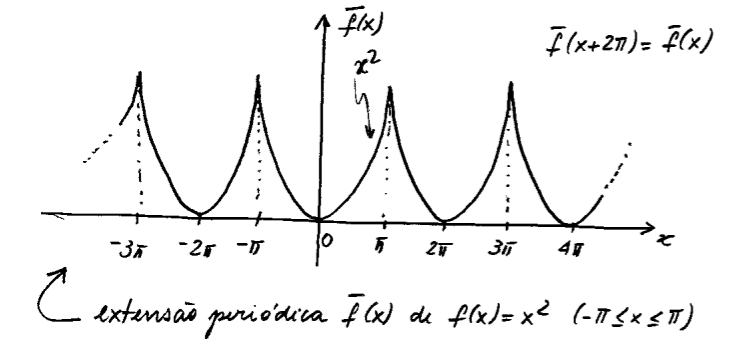
\includegraphics[width=0.8\textwidth]{figuras/01-0}
  \caption{Gráfico da série de Fourier para $f(x) = x^2$.}
  \label{fig:serie_fourier_grafico01}
\end{figure}

\begin{exem}
  Para
  \begin{dmath*}
    f(x) = \begin{cases}
      -1, & x < 0, \\
      +1, & x \geq 0.
    \end{cases}
  \end{dmath*}
  temos que
  \begin{dgroup*}
    \begin{dmath*}
      a_0 = \frac{1}{\pi} \int_{-\pi}^\pi f(x) \vi{x}
      = \frac{1}{\pi} \left[ -\int_\pi^0 \vi{x} + \int_0^\pi \vi{x} \right]
      = 0,
    \end{dmath*}
    \begin{dmath*}
      a_n = \frac{1}{\pi} \int_{-\pi}^\pi f(x) \cos\left( n x \right) \vi{x}
      = \frac{1}{n} \left[ -\int_{-\pi}^0 \cos\left( n x \right) \vi{x} +
      \int_0^\pi \cos\left( n x \right) \vi{x} \right]
      = 0,
    \end{dmath*}
    \begin{dmath*}
      b_n = \frac{1}{\pi} \int_{-\pi}^\pi f(x) \sin\left( n x \right) \vi{x}
      = \frac{1}{\pi} \left[ -\int_{-\pi}^0 \sin\left( n x \right) \vi{x} +
      \int_0^\pi \sin\left( n x \right) \vi{x} \right]
      = \frac{2}{\pi} \int_0^\pi \sin\left( n x \right) \vi{x}
      = \left. \frac{-2 \cos\left( n x \right)}{n \pi} \right|_0^\pi
      = \frac{-2}{n \pi} \left[ (-1)^n - 1 \right]
      = \begin{cases}
        0, & n \text{ é par}, \\
        4 / \left( n \pi \right), & n \text{ é ímpar}.
      \end{cases}
    \end{dmath*}
  \end{dgroup*}

  Logo,
  \begin{dmath*}
    f(x) = \sum_{n = 1}^\infty b_n \sin\left( n x \right)
    = \sum_{k = 1}^\infty b_{k + 1} \sin\left( (2k + 1) x \right)
    = \sum_{k = 0}^\infty \frac{4}{\left( 2k + 1 \right) \pi} \sin\left( (2k + 1) x \right).
  \end{dmath*}
\end{exem}

\begin{figure}[!htb]
  \centering
  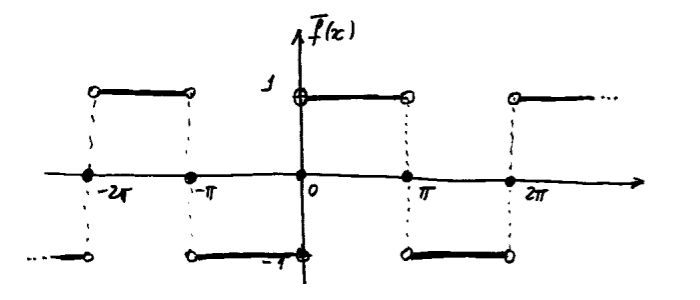
\includegraphics[width=0.8\textwidth]{figuras/01-1}
    % TODO Arrumar o comando \caption abaixo.
  \caption{Gráfico da série de Fourier para }
  \label{fig:serie_fourier_grafico02}
\end{figure}

Pela Figura~\ref{fig:serie_fourier_grafico02} que
\begin{dmath*}
  \bar{f}(x) = \begin{cases}
    1, & 0 < x < \pi, \\
    0, & x = 0, \pi, -\pi, \\
    -1, & -\pi < x < 0.
  \end{cases}
\end{dmath*}
e
\begin{dmath*}
  \bar{f}(x + 2 \pi) = \bar{f}(x).
\end{dmath*}

\begin{obs}
  $\bar{f}(0) \neq f(0)$, o que é característico do comportamento da série de
  Fourier em uma descontinuidade. Note que
  \begin{dmath*}
    \bar{f}(0) = \frac{1}{2} \left[ \lim_{x \to 0^+} f(x) + \lim_{x \to 0^-}
    f(x) \right]
  \end{dmath*}
  nesse caso (que se mostrará verdade no caso geral!).
\end{obs}

\begin{defi}
  Seja $\mathcal{L}^2[a, b]$ o conjunto das funções de quadrado integrável em $a
  \leq x \leq b$. Dizemos que $f(x)$ e $g(x)$ são ortogonais nesse intervalo se
  \begin{dmath*}
    \int_a^b f(x) g(x) \vi{x} = 0.
  \end{dmath*}
\end{defi}

\begin{obs}
  Lembrando que
  \begin{dmath*}
    0 \leq \left( f - g \right)^2 = f^2 + g^2 - 2 f g,
  \end{dmath*}
  ou seja,
  \begin{dmath*}
    2 f g \leq f^2 + g^2,
  \end{dmath*}
  concluímos que se $f, g \in \mathcal{L}^2[a, b]$, então existe $\int_a^b f(x)
  g(x) \vi{x}$. Além disso,
  \begin{dmath*}
    \left( f + g \right)^2 = f^2 + g^2 + 2 f g \leq 2 \left( f^2 + g^2 \right),
  \end{dmath*}
  o que garante que $f + g \in \mathcal{L}^2[a, b]$. Como $\mathcal{L}^2[a, b]$
  é um espaço vetorial, podemos pensar nessa integral como o produto escalar
  $<f, g>$ de $f, g \in \mathcal{L}^2[a, b]$:
  \begin{dmath*}
    \langle f, g \rangle = \int_a^b f(x) g(x) \vi{x}.
  \end{dmath*}
\end{obs}

\begin{prop}
  O conjunto $\left\{ 1, \cos\left( n x \right), \sin\left( n x \right)
  \right\}$ ($n = 1, 2, \ldots$) é ortogonal em $[-\pi, \pi]$.
\end{prop}
\begin{proof}
  Devemos mostrar que
  \begin{dgroup}
    \begin{dmath}[label={eq:serie_fourier_ort01}]
      \int_{-\pi}^\pi 1 \cos\left( n x \right) \vi{x} = \int_{-\pi}^\pi 1 \sin
      \left( n x \right) \vi{x} = 0,
    \end{dmath}
    \begin{dmath}[label={eq:serie_fourier_ort02}]
      \int_{-\pi}^\pi \cos\left( n x \right) \cos\left( m x \right) \vi{x} =
      \int_{-\pi}^\pi \sin\left( n x \right) \sin\left( m x \right) \vi{x} = 0
      \condition{$n \neq m$,}
    \end{dmath}
    \begin{dmath}[label={eq:serie_fourier_ort03}]
      \int_{-\pi}^\pi \cos\left( n x \right) \sin\left( m x \right) \vi{x} = 0.
    \end{dmath}
  \end{dgroup}
  As integrais \eqref{eq:serie_fourier_ort01} são triviais. Quanto a
  \eqref{eq:serie_fourier_ort02} e \eqref{eq:serie_fourier_ort03}, elas são
  calculadas de forma análoga, de modo que faremos explicitamente apenas uma
  delas. Usando a identidade
  \begin{dmath*}
    \cos\left( n x \right) \cos\left( m x \right) = \frac{1}{2} \cos\left( (n -
    m) x \right) + \frac{1}{2} \cos\left( (n + m) x \right)
  \end{dmath*}
  segue, para $n \neq m$, que
  \begin{dmath*}
    \int_{-\pi}^\pi \cos\left( n x \right) \cos\left( m x \right) \vi{x} =
    \frac{1}{2} \left. \frac{\sin\left( (n - m) x \right)}{n - m}
    \right|_{-\pi}^\pi + \frac{1}{2} \left. \frac{\sin\left( (n + m) x
    \right)}{n - m} \right|_{-\pi}^\pi = 0
  \end{dmath*}
  pois $\sin\left( k \pi \right) = 0$ para $k$ inteiro.

  Não custa chamar a atenção para o fato que \eqref{eq:serie_fourier_ort03} vale
  para quaisquer $n$ e $m$, enquanto \eqref{eq:serie_fourier_ort02} vale para $n
  \neq m$. Quando $n = m$, para \eqref{eq:serie_fourier_ort02} temos
  \begin{dmath*}
    \int_{-\pi}^\pi \cos^2\left( n x \right) \vi{x} = \int_{-\pi}^\pi
    \sin^2\left( n x \right) \vi{x} = \pi.
  \end{dmath*}
\end{proof}

\begin{teo}
  Se uma série trigonométrica converge uniformemente para a função $f(x)$ em
  $-\pi \leq x \leq \pi$, então ela é a série de Fourier de $f(x)$.
\end{teo}
\begin{proof}
  Se
  \begin{dmath*}
    f(x) = \frac{A_0}{2} + \sum_{n = 1}^\infty \left( A_n \cos\left( n x \right)
    + B_n \sin\left( n x \right) \right)
  \end{dmath*}
  converge uniformemente, o mesmo acontecerá com a série multiplicada por
  $\cos\left( m x \right)$ ou $\sin\left( m x \right)$. Como uma série
  uniformemente convergente pode ser integrada termo a termo, temos, por exemplo
  \begin{dmath*}
      \int_{-\pi}^\pi f(x) \cos\left( m x \right) \vi{x} = \frac{A_0}{2}
      \underbrace{\int_{-\pi}^\pi \cos\left( m x \right) \vi{x}}_{= 0} + \sum_{n
      = 1}^\infty \left( A_n \underbrace{\int_{-\pi}^\pi \cos\left( n x \right)
      \cos\left( m x \right) \vi{x}}_{= 0 (n \neq m)} + B_n
      \underbrace{\int_{-\pi}^\pi \sin\left( n x \right) \cos\left( m x \right)
      \vi{x}}_{= 0} \right)
  \end{dmath*}
  onde usamos a proposição anterior, de modo que
  \begin{dmath*}
    \int_{-\pi}^\pi f(x) \cos\left( m x \right) \vi{x} = A_m \int_{-\pi}^\pi
    \cos^2\left( m x \right) \vi{x} = \pi A_m,
  \end{dmath*}
  ou seja, $A_m$ é um coeficiente de Fourier. Procedendo de forma análogo,
  veremos que o mesmo acontece com $A_0$ e $B_m$, de modo que se trata de uma
  série de Fourier.
\end{proof}

\section{Mudança de intervalo}
Vamos agora, ao invés de $T = 2 \pi$, considerar um período $T = 2 L$. Para
isso, na série de Fourier
\begin{dmath*}
  f(x') = \frac{a_0}{2} + \sum_{n = 1}^\infty \left( a_n \cos\left( n x' \right)
  + b_n \sin\left( n x' \right) \right),
\end{dmath*}
vamos fazer a mudança de variável
\begin{dmath*}
  x' = \frac{\pi}{L} x.
\end{dmath*}
Assim, para $f(x') = f(\pi x / L) = f(x)$, temos
\begin{dmath*}
  F(x) = \frac{a_0}{2} + \sum_{n = 1}^\infty \left( a_n \cos\left( \frac{n \pi
  x}{L} \right) + b_n \sin\left( \frac{n \pi x}{L} \right) \right),
\end{dmath*}
com
\begin{dmath*}
  a_n = \frac{1}{\pi} \int_{-\pi}^\pi f(x') \cos\left( n x' \right) \vi{x'} =
  \frac{1}{\pi} \int_{-L}^L \frac{\pi}{L} f\left( \frac{\pi}{L} x \right)
  \cos\left( \frac{n \pi x}{L} \right) \vi{x},
\end{dmath*}
ou seja,
\begin{dmath*}
  a_n = \frac{1}{L} \int_{-L}^L F(x) \cos\left( \frac{n \pi x}{L} \right)
  \vi{x} \condition{$ n = 1, 2, \ldots$}
\end{dmath*}
e da mesma forma
\begin{dmath*}
  b_n = \frac{1}{L} \int_{-L}^L F(x) \sin\left( \frac{n \pi x}{L} \right)
  \vi{x} \condition{$n = 1, 2, \ldots$}
\end{dmath*}

\begin{exem}
  Para $f(x) = x^2, - 2 \pi \leq x \leq 2 \pi$ temos, usando $L = 2 \pi$
  (portanto período $T = 4\pi$), encontramos que
  \begin{dmath*}
    x^2 = \frac{4 \pi^2}{3} + \sum_{n = 1}^\infty \frac{16 (-1)^n}{n^2}
    \cos\left( \frac{n x}{2} \right).
  \end{dmath*}
\end{exem}

\section{Forma complexa}
Temos que $\exp(i x) = \cos(x) + i \sin(x)$ e portanto
\begin{dgroup*}
  \begin{dmath*}
    \cos\left( \frac{n \pi x}{L} \right) = \frac{1}{2} \left( \exp\left( i
    \frac{n \pi x}{L} \right) + \exp\left( -i \frac{n \pi x}{L} \right) \right),
  \end{dmath*}
  \begin{dmath*}
    \sin\left( \frac{n \pi x}{L} \right) = \frac{1}{2 i} \left( \exp\left( i
    \frac{n \pi x}{L} \right) - \exp\left( -i \frac{n \pi x}{L} \right) \right).
  \end{dmath*}
\end{dgroup*}
Logo,
\begin{dmath*}
  f(x) = \frac{a_0}{2} + \sum_{n = 1}^\infty \left[ \frac{a_n}{2} \exp\left( i
  \frac{n \pi x}{L} \right) + \frac{a_n}{2} \exp\left( -i \frac{n \pi x}{L}
  \right) - \frac{b_n i}{2} \exp\left( i \frac{n \pi x}{L} \right) + \frac{b_n
  i}{2} \exp\left( -i \frac{n \pi x}{L} \right) \right]
  = \frac{a_0}{2} + \sum_{n = 1}^\infty \underbrace{\left( \frac{a_n - i b_n}{2}
  \right)}_{c_n} \exp\left( i \frac{n \pi x}{L} \right) + \sum_{n = 1}^\infty
  \underbrace{\left( \frac{a_n + i b_n}{2} \right)}_{c_n^*} \exp\left( -i
  \frac{n \pi x}{L} \right)
\end{dmath*}

\begin{defi}
  Temos que $c_{- n} = c_n^*$, portanto
  \begin{dmath*}
    c_n = \begin{cases}
      \left( 1/2 \right) \left( a_n - i b_n \right), & n = 1, 2, \ldots \\
      \left( 1/2 \right) \left( a_n + i b_n \right), & n = -1, -2, \ldots \\
      \left( 1/2 \right) a_0, & n = 0.
    \end{cases}
  \end{dmath*}
  Logo,
  \begin{dmath*}
    f(x) = c_0 + \sum_{n = 1}^\infty c_n \exp\left( i (n \pi x) / L \right) +
    \sum_{n = -1}^{-\infty} \underbrace{\left( 1/2) \right) \left( a_{-n} + i
    b_{-n} \right)}_{c_n} \exp\left( i (n \pi x) / L \right)
    = \sum_{n = -\infty}^\infty c_n \exp\left( i (n \pi x) / L \right).
  \end{dmath*}
\end{defi}

\begin{obs}
  Note que
  \begin{dmath*}
    f^*(x) = \sum_{n = -\infty}^\infty c_n^* \exp\left( -i n \pi x / L \right)
    = \sum_{n = -\infty}^`9 c_{-n}^* \exp\left( i n \pi x / L \right)
    = \sum_{n = -\infty}^\infty c_n \exp\left( i n \pi x / L \right)
    = f(x).
  \end{dmath*}
\end{obs}

E $c_n$ é obtido por
\begin{dmath*}
  \int_{-L}^L \exp\left( \frac{-i m \pi x}{L} \right) \exp\left( \frac{i n \pi
  x}{L} \right)
  \vi{x} = \int_{-L}^L \exp\left( i (n - m) \pi x / L \right) \vi{x}
  = \begin{cases}
    \int_{-L}^L \vi{x} = 2 L, & n = m, \\
    \left. \exp\left( \frac{i (n - m) \pi x}{L} \right) \left( \frac{i (n - m)
    \pi}{L} \right)^{-1} \right\vert_{-L}^L = 0,
  \end{cases}
  = 2 L \delta_{mn}.
\end{dmath*}
Com isso
\begin{dmath*}
  \int_{-L}^L f(x) \exp\left( \frac{-i m \pi x}{L} \right) \vi{x} = \sum_{n =
  -\infty}^{\infty} c_n \int_{-L}^L \exp\left( i n \pi x / L \right) \exp\left( -i
  m \pi x / L \right) \vi{x}
  = 2 L \sum_{n = \infty}^{\infty} c_n \delta_{mn}
  = 2 L c_m.
\end{dmath*}
Logo,
\begin{dmath*}
  c_n = \frac{1}{2L} \int_{-L}^L f(x) \exp\left( -i n \pi x / L \right) \vi{x}.
\end{dmath*}

\begin{exem}
  Seja $f(x)$ dado por
  \begin{dmath*}
    f(x) = \begin{cases}
      1 / 2a, & |x| \leq a, \\
      0, & |x| > a,
    \end{cases}
  \end{dmath*}
  onde $a < L$. Logo, temos
  \begin{dmath*}
    c_n = \frac{1}{2L} \int_{-L}^L f(x) \exp\left( -i n \pi x / L \right) \vi{x}
    = \frac{1}{2L} \int_{-a}^a \frac{1}{2a} \exp\left( -i n \pi x / L \right)
    = \frac{1}{2L} \frac{1}{2a} \left. \frac{\exp\left( -i n \pi x / L
    \right)}{- i n \pi / L} \right|_{-a}^a
    = \frac{1}{2 (2a) (-i n \pi)} \left( \exp\left( -i n \pi a / L \right) -
    \exp\left( i n \pi a / L \right) \right)
    = \frac{1}{2 a n \pi} \left( \frac{\exp\left( i n \pi a / L \right) -
    \exp\left( -i n \pi a / L \right)}{2 i} \right)
    = \sin\left( n \pi a / L \right) \left( 2 n \pi a \right)^{-1}.
  \end{dmath*}
  E portanto,
  \begin{dmath*}
    f(x) = \sum_{n = -\infty}^\infty \frac{\sin\left( n \pi a / L \right)}{2 n
    \pi a} \exp\left( i n \pi a / L \right).
  \end{dmath*}
  Também é possível
  \begin{dmath*}
    f(x) = \frac{1}{2 L} + \sum_{n = 1}^\infty \frac{\sin\left( n \pi a / L
    \right)}{2 n \pi a} \exp\left( i n \pi a / L \right) + \sum_{n = 1}^\infty
    \frac{\sin\left( (-n) \pi a / L \right)}{2 (-n) \pi a} \exp\left( i (-n) \pi
    a / L \right)
    = \frac{1}{2L} + \sum_{n = 1}^\infty \frac{\sin\left( n \pi a / L \right)}{2
    n \pi a} \left( \exp\left( i n \pi a / L \right) + \exp\left( -i n \pi a / L
    \right) \right)
    = \frac{1}{2L} + \sum_{n = 1}^\infty \frac{\sin\left( n \pi a / L \right)}{n
    \pi a} \cos\left( n \pi a / L \right).
  \end{dmath*}
\end{exem}

\section{Propriedades de Paridade: Séries em Seno e Cosseno}
Temos, por definição que
\begin{dmath*}
  f(-x) = \begin{cases}
    f(x) \Rightarrow f \text{ é par}, \\
    -f(x) \Rightarrow f \text{ é ímpar}.
  \end{cases}
\end{dmath*}
Debotando uma função par por $f_+(x)$ e uma função ímpar por $f_-(x)$ temos
\begin{dmath*}
  f_\pm(-x) = \pm f_\pm(x).
\end{dmath*}

\begin{prop}
  Temos que
  \begin{dmath*}
    \int_{-L}^L f(x) \vi{x} = \begin{cases}
      2 \int_0^L f(x) \vi{x}, & f \text{ é par}, \\
      0, & f \text{ é ímpar}.
    \end{cases}
  \end{dmath*}
\end{prop}
\begin{proof}
  Temos que
  \begin{dmath*}
    \int_{-L}^L f_\pm(x) \vi{x} = \int_{-L}^0 f_\pm(x) \vi{x} + \int_0^L f_\pm(x) \vi{x}
    = -\int_{-L}^0 f_\pm(-x) \vi{x} + \int_0^L f_\pm(x) \vi{x}
    = \int_0^L f_\pm(-x) \vi{x} + \int_0^L f_\pm(x) \vi{x}
    = \pm \int_0^L f_\pm(x) \vi{x} + \int_0^L f_\pm(x) \vi{x}
    = \begin{cases}
      2 \int_0^L f_\pm(x) \vi{x}, & \text{para } f_+, \\
      0, & \text{para } f_-.
    \end{cases} \qedhere
  \end{dmath*}
\end{proof}

Por outro lado, é fácil verificar as informações da tabela abaixo.
\begin{table}[htb]
  \centering
  \begin{tabular}{|c|c|c|}
    \hline
    $f(x)$ & $g(x)$ & $f(x) g(x)$ \\ \hline
    par & par & par \\ \hline
    ímpar & par & ímpar \\ \hline
    ímpar & ímpar & par \\ \hline
  \end{tabular}
\end{table}

Logo, da proposição:
\begin{dmath*}
  a_n = \frac{1}{L} \int_{-L}^L f(x) \cos\left( n \pi x / L \right) \vi{x} = 0
\end{dmath*}
se $f(x)$ é ímpar e
\begin{dmath*}
  b_n = \frac{1}{L} \int_{-L}^L f(x) \sin\left( n \pi x / L \right) \vi{x} = 0
\end{dmath*}
se $f(x)$ é par.

Logo:
\begin{enumerate}
  \item se $f(x) = f_+(x)$ é par:
    \begin{dgroup*}
      \begin{dmath*}
        f_+(x) = \frac{a_0}{2} + \sum_{n = 1}^\infty a_n \cos\left( n \pi x / L \right),
      \end{dmath*}
      \begin{dmath*}
        a_n = \frac{2}{L} \int_0^L f(x) \cos\left( n \pi x / L \right) \vi{x}
      \end{dmath*}
    \end{dgroup*}
    que é a Série de Fourier em cossenos.
  \item Se $f(x) = f_-(x)$ é ímpar:
    \begin{dgroup*}
      \begin{dmath*}
        f_-(x) = \sum_{n = 1}^\infty n_n \sin\left( n \pi x / L \right),
      \end{dmath*}
      \begin{dmath*}
        b_n = \frac{2}{L} \int_0^L f(x) \sin\left( n \pi x / L \right) \vi{x}
      \end{dmath*}
    \end{dgroup*}
    que é a Série de Fourier em senos.
\end{enumerate}

\begin{exem}
  Considere $f(x) = x / \left( 2 L \right) + 1 / 2$ cujo gráfico é ilustrado
  abaixo.
  \begin{center}
    \begin{tikzpicture}[scale=2]
      \draw[->] (-1.6,0) -- (-1,0) node[below]{$-L$} -- (1,0) node[below]{$L$}
      -- (1.6,0);
      \draw[->] (0,-.5) -- (0,.5) node[left]{$1/2$} -- (0,1) node[left]{$1$} --
      (0,1.5);
      \draw (-1.5,-.25) -- (-1,0) -- (0,.5) -- (1,1) -- (1.5,1.25)
      node[right]{$f(x)$};
      \draw[dotted] (0,1) rectangle (1,0);
    \end{tikzpicture}
  \end{center}
  \begin{enumerate}
    \item Série de Fourier:
      \begin{dgroup*}
        \begin{dmath*}
          a_0 = \frac{1}{L} \int_{-L}^L \left( \frac{x}{2 L} + \frac{1}{2}
          \right) \vi{x}
          = \left. \frac{1}{L} \left( \frac{x^2}{4 L} + \frac{x}{2} \right)
          \right|_{-L}^L
          = 1,
        \end{dmath*}
        \begin{dmath*}
          a_n = \frac{1}{L} \int_{-L}^L \cos\left( n \pi x / L \right) \left(
          \frac{x}{2 L} + \frac{1}{2} \right) \vi{x}
          = \frac{1}{2 L^2} \int_{-L}^L x \cos\left( n \pi x / L \right) \vi{x}
          + \frac{1}{2L} \int_{-L}^L \cos\left( n \pi x / L \right) \vi{x}
          = 0,
        \end{dmath*}
        \begin{dmath*}
          b_n = \frac{1}{L} \int_{-L}^L \sin\left( n \pi x / L \right) \left(
          \frac{x}{2L} + \frac{1}{2} \right) \vi{x}
          = \frac{1}{2L^2} \int_{-L}^L x \sin\left( n \pi x / L \right) \vi{x} +
          \frac{1}{2L} \int_{-L}^L \sin\left( n \pi x / L \right) \vi{x}
          = \frac{1}{2L^2} \left[ \left. \frac{-x \cos\left( n \pi x / L
          \right)}{n \pi / L} \right|_{-L}^L + \frac{1}{n \pi / L} \int_{-L}^L
          \cos\left( n \pi x / L \right) \right]
          = \frac{1}{2L^2} \frac{\left( -2L^2 \right) \left( -1 \right)^n}{n
          \pi}
          = \frac{(-1)^{n + 1}}{n \pi}.
        \end{dmath*}
      \end{dgroup*}
      Logo,
      \begin{dmath*}
        F(x) = \frac{1}{2} + \sum_{n = 1}^\infty \frac{(-1)^{n + 1}}{n \pi}
        \sin\left( n \pi x / L \right).
      \end{dmath*}
      \begin{center}
        \begin{tikzpicture}[scale=2]
          \draw[->] (-3.2,0) -- (3.2,0);
          \draw[->] (0,-.5) -- (0,.5) node[left]{$1/2$} -- (0,1) node[left]{$1$}
          -- (0,1.5);
          \foreach \x in {-3,-1,1}{
          \draw (\x,0) -- ++(1,.5) -- ++(1,.5);
          }
          \foreach \x in {-3,-2,...,3}{
          \draw (\x,0) node[below]{$\x L$};
          }
        \end{tikzpicture}
      \end{center}

    \item Série de Fourier em senos:
      \begin{dmath*}
        b_n = \frac{2}{L} \int_0^L \sin\left( n \pi x / L \right) \left(
        \frac{x}{2} + \frac{1}{2} \right) \vi{x}
        = \frac{1}{L^2} \int_0^L x \sin\left( n \pi x / L \right) \vi{x} +
        \frac{1}{L} \int_0^L \sin\left( n \pi x / L \right) \vi{x}
        = \frac{1}{L^2} \left[ \left. \frac{- x \cos\left( n \pi x / L
        \right)}{n \pi / L} \right|_0^L + \frac{L}{n \pi} \int_0^L \cos\left( n
        \pi x / L \right) \vi{x} \right] + \frac{1}{L} \left. \frac{- \cos\left(
        n \pi x / L \right)}{n \pi / L} \right|_0^L
        = \frac{-1}{n \pi} \cos\left( n \pi \right) - \frac{1}{n \pi} \cos\left(
        n \pi \right) + \frac{1}{n \pi}
        = \frac{1 - 2 (-1)^n}{n \pi}.
      \end{dmath*}
      Logo,
      \begin{dmath*}
        F_-(x) = \sum_{n = 1}^\infty \left( \frac{1 - 2 (-1)^n}{n \pi} \right)
        \sin\left( n \pi x / L \right).
      \end{dmath*}
            % TODO Incluir gráfico.

    \item Série de Fourier em cossenos:
      \begin{dgroup*}
        \begin{dmath*}
          a_0 = \frac{2}{L} \int_0^L \left( \frac{x}{2L} + \frac{1}{2} \right) \vi{x}
          = \frac{2}{L} \left. \left( \frac{x^2}{4 L} + \frac{x}{2} \right) \right|_0^L
          = \frac{3}{2},
        \end{dmath*}
        \begin{dmath*}
          a_n = \frac{2}{L} \int_0^L \left( \frac{x}{2L} + \frac{1}{2} \right)
          \cos\left( n \pi x / L \right)
          = \frac{1}{L^2} \int_0^L x \cos\left( n \pi x / L \right) \vi{x} +
          \frac{1}{L} \int_0^L \cos\left( n \pi x / L \right) \vi{x}
          = \frac{1}{L^2} \left[ \left. \frac{x \sin\left( n \pi x / L
          \right)}{n \pi / L} \right|_0^L - \frac{L}{n \pi} \int_0^L \sin\left(
          n \pi x / L \right) \vi{x} \right] + \frac{1}{L} \frac{1}{n \pi / L}
          \left. \sin\left( n \pi x / L \right) \right|_0^L
          = \frac{1}{L n \pi} \left. \frac{\cos\left( n \pi x / L \right)}{n
          \pi / L} \right|_0^L
          = \frac{1}{n^2 \pi^2} \left[ (-1)^n - 1 \right].
        \end{dmath*}
      \end{dgroup*}
      Logo,
      \begin{dmath*}
        F_+(x) = \frac{3}{4} + \sum_{n = 1}^\infty \frac{\left[ (-1)^n - 1
        \right]}{n^2 \pi^2} \cos\left( n \pi x / L \right).
      \end{dmath*}
            % TODO Incluir gráfico.
  \end{enumerate}
\end{exem}

\section{Teorema de Fourier}
Para facilitar a notação, vamos tomar $L = \pi$. Então
\begin{dmath*}
  f(x) = \frac{a_0}{2} + \sum_{n = 1}^\infty \left( a_n \cos\left( n x \right) +
  b_n \sin\left( n x \right) \right)
  = \frac{1}{2} \left[ \frac{1}{\pi} \int_{-\pi}^\pi f(\xi) \vi{\xi} \right] +
  \sum_{n = 1}^\infty \left[ \left( \frac{1}{\pi} \int_{-\pi}^\pi f(\xi)
  \cos\left( n \xi \right) \vi{\xi} \right) \cos\left( n x \right) + \left(
  \frac{1}{\pi} \int_{-\pi}^\pi f(\xi) \sin\left( n \xi \right) \vi{\xi} \right)
  \sin\left( n x \right) \right]
  = \frac{1}{2\pi} \int_{-\pi}^\pi f(\xi) \vi{\xi} + \frac{1}{\pi} \sum_{n =
  1}^\infty \int_{-\pi}^\pi f(\xi) \left[ \cos\left( n \xi \right) \cos\left( n
  x \right) + \sin\left( n \xi \right) \sin\left( n x \right) \right] \vi{\xi}.
\end{dmath*}
Portanto,
\begin{dmath}[label={eq:serie_fourier}]
  f(x) = \frac{1}{2\pi} \int_{-\pi}^\pi f(\xi) \vi{\xi} + \frac{1}{\pi} \sum_{n
  = 1}^\infty \int_{-\pi}^\pi f(\xi) \cos\left( n (\xi - x) \right) \vi{\xi}.
\end{dmath}

\begin{teo}[Fourier] \label{teo:fourier}
  Seja $f(x)$ uma função contínua por partes e com derivadas laterais no
  intervalo $(-\pi, \pi)$ e periódica com período $2\pi$. Então sua série de
  Fourier, \eqref{eq:serie_fourier}, converge para o valor
  \begin{dmath*}
    \frac{1}{2} \left[ f(x + 0) + f(x - 0) \right]
  \end{dmath*}
  em $-\infty < x < \infty$.
\end{teo}

Antes de provarmos o teorema de Fourier precisamos explicitar o que entendemos
por derivadas laterais e provar alguns lemas auxiliares.

\subsection{Derivadas Laterais}
Seja
\begin{dgroup*}
  \begin{dmath*}
    f(x_0 + 0) = \lim_{x \to x_0^+} f(x),
  \end{dmath*}
  \begin{dmath*}
    f(x_0 - 0) = \lim_{x \to x_0^-} f(x).
  \end{dmath*}
\end{dgroup*}

\begin{defi}
  Derivada à direita, $f_+'(x_0)$:
  \begin{dmath*}
    f_+'(x_0) = \lim_{h \to 0} \frac{f(x_0 + h) - f(x_0 + 0)}{h} \condition{$h >
    0$.}
  \end{dmath*}
  Derivada à esquerda, $f_-'(x_0)$:
  \begin{dmath*}
    f_-'(x_0) = \lim_{h \to 0} \frac{f(x_0 - 0) - f(x_0 - h)}{h} \condition{$h >
    0$.}
  \end{dmath*}
\end{defi}
\begin{obs}
  Não confundir as notações: $f_+'$ ($f_-'$) não é a derivada de uma função par
  (ímpar).
\end{obs}
\begin{obs}
  Note o uso de $f(x_0 + 0)$ e $f(x_0 - 0)$ e não $f(x_0)$.
\end{obs}

Sejam $f, f'$ contínuas por partes e $[a,b]$ um intervalo onde $f$ e $f'$ são
contínuas e tem limites laterais. Portanto, em $[a,b]$ vale o teorema do valor
médio, i.e., $\exists \theta (0 < \theta < 1)$ tal que para $0 < \lambda < b -
1$ verifica-se que
\begin{dmath*}
  \frac{f(a + \lambda) - f(a + 0)}{\lambda} = f'(a + \theta \lambda).
\end{dmath*}
Então
\begin{dmath*}
  \lim_{\lambda \to 0} \frac{f(a + \lambda) - f(a + 0)}{\lambda} = f_+'(a) =
  \lim_{\lambda \to 0} f'(a + \theta \lambda) = f'(a + 0).
\end{dmath*}
Analogamente: $f_-'(b) = f'(b - 0)$.

Portanto, em cada ponto de um intervalo fechado no qual $f$ e $f'$ são contínuas
por partes, as derivadas laterais de $f$ (do interior do intervalo) existem e
são as mesmas que os correspondentes limites laterais de $f'$.
\begin{exem}
  Considere a função dada por
  \begin{dmath*}
    f(x) = \begin{cases}
      \sin(x), & x \geq 0, \\
      x^2, & x < 0.
    \end{cases}
  \end{dmath*}
  Então,
  \begin{dgroup*}
    \begin{dmath*}
      f_+'(0) = \lim_{h \to 0} \frac{\sin\left( h \right) - 0}{h} = 1,
    \end{dmath*}
    \begin{dmath*}
      f_-'(0) = \lim_{h \to 0} \frac{0 - \left( -h \right)^2}{h} = 0.
    \end{dmath*}
  \end{dgroup*}
  Portanto, $f'(x)$ é contínua por partes e $f_+'(0) = f'(0 + 0)$ e $f_-'(0) =
  f'(0 - 0)$.
\end{exem}
\begin{exem}
  Considere a função dada por
  \begin{dmath*}
    f(x) = \begin{cases}
      1, & x \geq 0, \\
      0, & x < 0.
    \end{cases}
  \end{dmath*}
  Então,
  \begin{dgroup*}
    \begin{dmath*}
      \lim_{\delta x \to 0^+} \frac{1 - 1}{\delta x} = 0,
    \end{dmath*}
    \begin{dmath*}
      \lim_{\delta x \to 0^-} \frac{0 - 1}{\delta x} = +\infty
    \end{dmath*}
  \end{dgroup*}
  de maneira que não existe $f'(0)$. Mas
  \begin{dgroup*}
    \begin{dmath*}
      f_+'(0) = \lim_{h \to 0} \frac{1 - 1}{h} = 0,
    \end{dmath*}
    \begin{dmath*}
      f_-'(0) = \lim_{h \to 0} \frac{0 - 0}{h} = 0.
    \end{dmath*}
  \end{dgroup*}
  Portanto, $f_+'(0) = f_-'(0) = 0$ mas não existe $f'(0)$.
\end{exem}
\begin{exem}
  Considere a função dada por
  \begin{dmath*}
    f(x) = \begin{cases}
      x^2 \sin\left( 1 / x \right), & x \neq 0, \\
      0, & x = 0.
    \end{cases}
  \end{dmath*}
  Então,
  \begin{dmath*}
    \lim_{x \to 0} x^2 \sin\left( 1 / x \right) = \lim_{x \to 0} x \sin\left( 1
    / x \right) \left( 1 / x \right)^{-1} = 0
  \end{dmath*}
  e
  \begin{dgroup*}
    \begin{dmath*}
      f_+'(0) = \lim_{h \to 0} \frac{h^2 \sin\left( 1 / h \right) - 0}{h} = 0,
    \end{dmath*}
    \begin{dmath*}
      f_-'(0) = \lim_{h \to 0} \frac{0 - (-h)^2 \sin\left( 1 / (-h) \right)}{h}
      = 0.
    \end{dmath*}
  \end{dgroup*}
  Portanto, $f'(x) = 2 x \sin\left( 1 / x \right) - \cos\left( 1 / x \right)$
  que implica não existir $f'(0+)$ e nem $f'(0-)$ de maneira que não existe
  $f'(0)$. Neste caso, $f_+'(0) \neq f'(0+)$ e $f_-'(0) \neq f'(0-)$.
\end{exem}

\subsection{Lemas auxiliares}
\begin{lem} \label{lem:cont}
  Se $F$ é contínua por partes em $[a,b]$, então
  \begin{enumerate}
    \item \label{enum:cont:sin} $\lim_{k \to \infty} \int_a^b F(x) \sin\left( k
      x \right) \vi{x} = 0$,
    \item \label{enum:cont:cos} $\lim_{k \to \infty} \int_a^b F(x) \cos\left( k
      x \right) \vi{x} = 0$.
  \end{enumerate}
\end{lem}
\begin{proof}
  Vamos dividir $(a,b)$ em intervalos onde $F$ é contínua. Vamos denotar um
  desses intervalos por $[p,q]$. Então vale o item~\ref{enum:cont:sin} se
  \begin{dmath*}
    I = \lim_{k \to \infty} \int_p^q F(x) \sin\left( k x \right) \vi{x} = 0.
  \end{dmath*}
    % TODO Terminar a demonstração do Lema.
\end{proof}

\begin{lem} \label{lem:sin(x)/x}
  $\int_0^\infty \sin\left( x \right) / x \vi{x} = \pi / 2$.
\end{lem}
\begin{proof}
  Temos que
  \begin{dmath*}
    \int_0^\infty \frac{\sin\left( x \right)}{x} \vi{x} = F(0),
  \end{dmath*}
  onde $F(x) = \int_0^\infty \exp\left( -t x \right) \sin\left( x \right) / x
  \vi{x}$ para $t \geq 0$.

  Seja $S(x) = \sin\left( x \right) / x$.
    % TODO Terminar a demonstração do Lema.
\end{proof}

\begin{lem} \label{lem:F_+'(x)}
  Se $F$ é contínua por partes em $[0,b]$ e tem derivada à direita
  $F_+'(0)$, então
  \begin{dmath*}
    \lim_{k \to \infty} \int_0^b F(x) \frac{\sin\left( k x \right)}{x} \vi{x} =
    \frac{\pi}{2} F(0+).
  \end{dmath*}
\end{lem}
\begin{proof}
  Temos que
  \begin{dmath*}
    I(k) = \int_0^b F(x) \frac{\sin\left( k x \right)}{x} \vi{x}
    = \lim_{k \to \infty} \int_0^{k b} \frac{\sin\left( t \right)}{t} \vi{t}
    = \int_0^\infty \frac{\sin\left( t \right)}{t} \vi{t}
    \intertext{e pelo Lema~\ref{lem:sin(x)/x}}
    = \pi / 2.
  \end{dmath*}
    % TODO Terminar a demonstração do Lema.
\end{proof}

\begin{lem} \label{lem:lim_int}
  Seja $F$ uma função contínua por partes em $(a,b)$ e que tem derivadas
  laterias à esquerda e à direita em um ponto $x_0$ tal que $a < x_0 <
  b$. Então
  \begin{dmath*}
    \lim_{k \to \infty} \int_a^ F(x) \frac{\sin\left( k \left( x - x_0 \right)
    \right)}{x - x_0} \vi{x} = \pi \frac{F\left( x_0 + 0 \right) + F\left( x_0 -
    0 \right)}{2}.
  \end{dmath*}
\end{lem}
\begin{proof}
  Temos que
  \begin{dmath*}
    I(k) = \int_a^b F(x) \frac{\sin\left( k \left( x - x_0 \right) \right)}{x -
    x_0} \vi{x}
  \end{dmath*}
    % TODO Terminar a demonstração do Lema.
\end{proof}

\subsection{Demonstração do Teorema de Fourier}
De \eqref{eq:serie_fourier} na página \pageref{eq:serie_fourier}:
\begin{dmath*}
  f(x) = \frac{1}{\pi} \int_{-\pi}^{\pi} f(\epsilon) \left[
  \frac{1}{2} + \sum_{n = 1}^{\infty} \cos\left( n (\epsilon - x) \right)
  \right] \vi{\epsilon}
\end{dmath*}
de mod que a $N$-ésima soma parcial é
\begin{dmath*}
  S_N(x) = \frac{1}{\pi} \int_{-\pi}^{\pi} f(\epsilon) \left[
  \frac{1}{2} + \sum_{n = 1}^N \cos\left( n (\epsilon - x) \right) \right]
  \vi{\epsilon}.
\end{dmath*}
Por outro lado:
\begin{dmath*}
  \sum_{n = 1}^N \cos(n u) = \sum_{n = 1}^N \left( \frac{\exp(i n u) + \exp(-i n
  u)}{2} \right)
\end{dmath*}
e portanto
\begin{dmath*}
  2 \sum_{n = 1}^N \cos(n u) = \sum_{n = 1}^N \left( \exp(i u) \right)^n +
  \sum_{n = 1}^N \left( \exp(-i u) \right)^n
\end{dmath*}
mas $a^{N + 1} - 1 = (a - 1) (1 + a + a^2 + \ldots + a^N)$ que implica em
$\sum_{n = 0}^N a^n = (a^{N + 1} - 1) / (a - 1)$, para $a \neq 1$, e portanto
\begin{dmath*}
  2 \sum_{n = 1}^N \cos(n u) = \sum_{n = 0}^N \left( \exp(i n) \right)^n - 1 +
  \sum_{n = 0}^N \left( \exp(-i u) \right)^n - 1
  = \frac{(\exp(i u))^{N + 1} - 1}{\exp(i u) - 1} - 1 + \frac{(\exp(-i u))^{N +
  1} - 1}{\exp(-i u) - 1} - 1
  = \frac{\exp(i u (N + 1)) - 1 - \exp(+i u) + 1}{\exp(i u) - 1} +
  \frac{\exp(-i u (N + 1) - 1 - \exp(-i u) + 1}{\exp(-i u) - 1}
  = \frac{\exp(i u (N + 1)) - \exp(+i u)}{\exp(i u) - 1} +
  \frac{\exp(-i u (N + 1) - \exp(-i u)}{\exp(-i u) - 1}
  = \frac{\exp(i u (N + 1)) - \exp(+i u)}{\exp(i u / 2) \left( \exp(i u / 2) -
  \exp(-i u / 2) \right)} + \frac{\exp(-i u (N + 1) - \exp(-i u)}{\exp(-i u / 2)
  \left( \exp(-i u / 2) - \exp(i u / 2) \right)}
  = \frac{\exp(i u (N + 1 / 2)) - \exp(i u (1 - 1/2)) - \exp(-i u (N + 1 / 2)) +
  \exp(-i u (1 - 1/2))}{\exp(i u / 2) - \exp(-i u / 2)}
  = \frac{\exp(i u (N + 1 / 2)) - \exp(-i u (N + 1 / 2))}{\exp(i u / 2) -
  \exp(-i u / 2)} - \frac{\exp(i u / 2) - \exp(-i u / 2)}{\exp(i u / 2) -
  \exp(-i u / 2)}
  = \frac{\sin(N + 1 / 2) u}{\sin(u / 2)} - 1.
\end{dmath*}
Portanto,
\begin{dmath*}
  1 + 2 \sum_{n = 1}^N \cos(n u) = \frac{\sin(N + 1 / 2) u}{\sin(u / 2)}
\end{dmath*}
e
\begin{dmath*}
  S_N(x) = \int_{-\pi}^{\pi} f(\epsilon) \frac{\sin(N + 1 / 2) (\epsilon - x)}{2
  \pi \sin(\epsilon - x) / 2} \vi{\epsilon}
  = \int_{-\pi}^{\pi} f(\epsilon) D_N(\epsilon - x) \vi{\epsilon}.
\end{dmath*}

\begin{defi}
  O núcleo de Dirichlet, $D_N(u)$, é definido como
  \begin{dmath*}
    D_N(u) = \frac{\sin( (N + 1/2) u)}{2 \pi \sin(u / 2)}
  \end{dmath*}
  continuando \ldots

  Como $f(\epsilon)$ tem período $2 \pi$, assim como $\sin( (N + 1 / 2) u)$ e
  $\sin(u / 2)$, então $S_N(x)$ pode também ser escrito como
  \begin{dmath*}
    S_N(x) = \frac{1}{\pi} \int_a^{a + 2 \pi} f(\epsilon) \frac{\sin\left( (N +
    1/ 2) (\epsilon - x) \right)}{2 \sin\left( (\epsilon - x) / 2 \right)}
  \end{dmath*}
  onde escolhemos $a$ de modo que $a \leq x \leq a + 2 \pi$.

  Escrevendo:
  \begin{dmath*}
    S_N(x) = \frac{1}{\pi} \int_a^{a + 2 \pi} F(\epsilon) \frac{\sin\left( (N +
    1 / 2) (\epsilon - x) \right)}{\epsilon - x}
  \end{dmath*}
  onde
  \begin{dmath*}
    F(\epsilon) = f(\epsilon) \frac{(1 / 2) (\epsilon - x)}{\sin\left( (1 / 2)
    (\epsilon - x) \right)}
  \end{dmath*}
  e usando o Lema~\ref{lem:lim_int}:
  \begin{dgroup*}
    \begin{dmath*}
      \lim_{N \to \infty} S_N(x) = \frac{1}{\pi} \left[ \pi
      \frac{F(x + 0) + F(x - 0)}{2} \right],
    \end{dmath*}
    \begin{dmath*}
      F(x + 0) = \lim_{\epsilon \to x^{+}} F(\epsilon)
      = \lim_{\epsilon \to x^{+}} f(\epsilon) \lim_{\epsilon \to x^{+}}
      \frac{(1 / 2) (\epsilon - x)}{\sin\left( (1 / 2) (\epsilon - x) \right)}
      = \lim_{\epsilon \to x^{+}} f(\epsilon) 1
      = f(x + 0),
    \end{dmath*}
    \begin{dmath*}
      F(x - 0) = \lim_{\epsilon \to x^{-}} F(\epsilon)
      = \lim_{\epsilon \to x^{-}} f(\epsilon) \lim_{\epsilon \to x^{-}}
      \frac{(1 / 2) (\epsilon - x)}{\sin\left( (1 / 2) (\epsilon - x) \right)}
      = \lim_{\epsilon \to x^{-}} f(\epsilon) 1
      = f(x - 0)
    \end{dmath*}
  \end{dgroup*}
  e portanto
  \begin{dmath*}
    \lim_{N \to \infty} S_N(x) = \frac{f(x + 0) + f(x - 0)}{2}.
  \end{dmath*}
\end{defi}

\section{Convergência na Média}
Da expressão para o produto escalar em $\mathcal{L}^2(a, b)$ definimos uma norma
através de
\begin{dmath*}
  \| f \|^2 = <f, f> = \int_a^b \left[ f(x) \right]^2 \vi{x}.
\end{dmath*}

Com isso, dados as funções $f, g \in \mathcal{L}^2(a, b)$, definimos o desvio
total quadrático dessas funções como
\begin{dmath*}
  \Delta = \| f - g \|^2 = \int_a^b \left[ f(x) - g(x) \right]^2 \vi{x}.
\end{dmath*}

\begin{teo} \label{teo:min_desvio_total_quad}
  Seja o polinômio trigonométrico
  \begin{dmath*}
    \phi_N(x) = \frac{A_0}{2} + \sum_{n = 1}^N \left( A_n \cos\left( n x
    \right) + B_n \sin\left( n x \right) \right),
  \end{dmath*}
  onde $A_0$, $A_n$ e $B_n$ são indeterminados e $f(x)$ é uma função contínua
  por partes em $[-\pi, \pi]$. Então o desvio total quadrático $\Delta_N = \| f
  - \phi_N \|^2$ é minimizado quando os coeficientes $A_0$, $A_n$ e $B_n$ forem
  iguais aos coeficientes de Fourier de $f(x)$.
\end{teo}
\begin{proof}
  Temos que
  \begin{dmath*}
    \Delta_n = \int_{-\pi}^\pi \left[ f(x) - \phi_N(x) \right]^2 \vi{x}
    = \int_{-\pi}^\pi \left[ f(x) - \frac{A_0}{2} - \sum_{n = 1}^N \left( A_n
    \cos\left( n x \right) + B_n \sin\left( n x \right) \right) \right]^2 \vi{x}
    = \int_{-\pi}^\pi \left[ f(x) \right]^2 \vi{x} + \int_{-\pi}^\pi \left(
    \frac{A_0}{2}^2 \right) \vi{x} + \int_{-\pi}^\pi \sum_{n = 1}^N \sum_{m =
    1}^N A_n A_m \cos\left( n x \right) \cos\left( m x \right) \vi{x} +
    \int_{-\pi}^\pi \sum_{n = 1}^N \sum_{m = 1}^N B_n B_m \sin\left( n x
    \right) \sin\left( m x \right) \vi{x} - 2 \int_{-\pi}^\pi f(x)
    \frac{A_0}{2} \vi{x} - 2 \int_{-\pi}^\pi f(x) \sum_{n = 1}^N \cos\left( n
    x \right) \vi{x} - 2 \int_{-\pi}^\pi f(x) \sum_{n = 1}^N B_n \sin\left( n
    x \right) \vi{x} + 2 \int_{-\pi}^\pi \frac{A_0}{2} \cos\left( n x \right)
    \vi{x} + 2 \int_{-\pi}^\pi \frac{A_0}{2} \sum){n = 1}^N B_n \sin\left( n x
    \right) \vi{x} + 2 \int_{-\pi}^\pi \sum_{n = 1}^N \sum_{m = 1}^N A_n B_n
    \cos\left( n x \right) \sin\left( m x \right) \vi{x}
    = \int_{-\pi}^\pi \left[ f(x) \right]^2 \vi{x} + \frac{A_0^2}{4} 2 \pi +
    \sum_{n = 1}^N \sum_{m = 1}^N A_n A_m \underbrace{\int_{-\pi}^\pi \cos\left(
    n x \right) \cos\left( m x \right) \vi{x}}_{\pi \delta_{nm}} + \sum_{n =
    1}^N \sum_{m = 1}^N B_n B_m \underbrace{\int_{-\pi}^\pi \sin\left( n x
    \right) \sin\left( m x \right) \vi{x}}_{\pi \delta_{nm}} - A_0
    \int_{-\pi}^\pi f(x) \vi{x} - 2 \sum_{n = 1}^N A_n \int_{-\pi}^\pi f(x)
    \cos\left( n x \right) \vi{x} - 2 \sum_{n = 1}^N B_n \int_{-\pi}^\pi f(x)
    \sin\left( n x \right) \vi{x} + A_0 \sum_{n = 1}^N A_n
    \underbrace{\int_{-\pi}^\pi \cos\left( n x \right) \vi{x}}_{=0} + A_0
    \sum_{n = 1}^N B_n \underbrace{\int_{-\pi}^\pi \sin\left( n x \right)
    \vi{x}}_{=0} + 2 \sum_{n = 1}^N \sum_{m = 1}^N A_n B_m
    \underbrace{\int_{-\pi}^\pi \cos\left( n x \right) \sin\left( m x \right)
    \vi{x}}_{=0}
  \end{dmath*}
  Portanto,
  \begin{dmath*}
    \delta_N = \int_{-\pi}^\pi \left[ f(x) \right]^2 \vi{x} + \frac{\pi}{2}
    A_0^2 + \sum_{n = 1}^N \pi A_n^2 + \sum_{n = 1}^N \pi B_n^2 - A_0
    \int_{-\pi}^\pi f(x) \vi{x} - 2 \sum_{n = 1}^N A_n \int_{-\pi}^\pi f(x)
    \cos\left( n x \right) \vi{x} - 2 \sum_{n = 1}^N B_n \int_{-\pi}^\pi f(x)
    \sin\left( n x \right) \vi{x}
  \end{dmath*}
  Exigindo agora que
  \begin{dmath*}
    \devp{\Delta_N}{A_0} = \devp{\Delta_N}{A_n} = \devp{\Delta_N}{B_n} = 0
  \end{dmath*}
  para $n = 1, \ldots, N$ temos que
  \begin{dgroup*}
    \begin{dmath*}
      \devp{\Delta_N}{A_0} = \pi A_0 - \int_{-\pi}^\pi f(x) \vi{x} = 0
      \Rightarrow A_0 = \frac{1}{\pi} \int_{-\pi}^\pi f(x) \vi{x} = a_0,
    \end{dmath*}
    \begin{dmath*}
      \devp{\Delta_N}{A_n} = 2 \pi A_n - 2 \int_{-\pi}^\pi f(x) \cos\left( n x
      \right) \vi{x} = 0 \Rightarrow A_n = \frac{1}{\pi} \int_{-\pi}^\pi f(x)
      \cos\left( n x \right) \vi{x} = a_n,
    \end{dmath*}
    \begin{dmath*}
      \devp{\Delta_N}{B_n} = 2 \pi B_n - 2 \int_{-\pi} \pi f(x) \sin\left( n x
      \right) \vi{x} = 0 \Rightarrow B_n = \frac{1}{\pi} \int_{-\pi}^\pi f(x)
      \sin\left( n x \right) \vi{x} = b_n.
    \end{dmath*}
  \end{dgroup*}
  Além disso, é fácil ver que o extremo em questão é um mínimo.
\end{proof}

Com isso, temos que $\Delta_n^{\min}$ é dado por
\begin{dmath*}
  \Delta_N^{\min} = \int_{-\pi}^\pi \left[ f(x) \right]^2 \vi{x} + \frac{\pi}{2}
  a_0^2 + \sum_{n = 1}^N \pi a_n^2 + \sum_{n = 1}^N \pi b_k^2 - a_0 \left( \pi
  a_0 \right) - 2 \sum_{n = 1}^N a_n \left( \pi a_n \right) - 2 \sum_{n = 1}^N
  b_n \left( \pi b_n \right)
\end{dmath*}
e portanto
\begin{dmath*}
  \Delta_N^{\min} = \int_{-\pi}^\pi \left[ f(x) \right]^2 \vi{x} - \pi \left[
  \frac{a_0^2}{2} + \sum_{n = 1}^N \left( a_n^2 + b_n^2 \right) \right].
\end{dmath*}
Além disso, como $\Delta_N \geq 0$, temos que
\begin{dmath*}
  \frac{a_0^2}{2} + \sum_{n = 1}^N \left( a_n^2 + b_n^2 \right) \leq
  \frac{1}{\pi} \int_{-\pi}^\pi \left[ f(x) \right]^2 \vi{x}.
\end{dmath*}

\begin{prop}
  Os coeficientes de Fourier satisfazem a chamada desigualdade de Bessel:
  \begin{dmath*}
    \frac{a_0^2}{2} + \sum_{n = 1}^\infty \left( a_n^2 + b_n^2 \right) \leq
    \frac{1}{\pi} \int_{-\pi}^\pi \left[ f(x) \right]^2 \vi{x}.
  \end{dmath*}
\end{prop}
\begin{proof}
  Seja a sequência $\left\{ \Delta_N \right\}$, onde
  \begin{dmath*}
    \Delta_N = \frac{a_0^2}{2} + \sum_{n = 1}^N \left( a_n^2 + b_n^2 \right).
  \end{dmath*}
  Como consequência de $\Delta_n \geq 0$, temos acima que essa sequência é
  limitada. Além disso, ela é evidentemente monótona. Como uma sequencia
  monótona e limitada é convergente, segue que existe $\lim_{N \to \infty}
  \Delta_N$ satisfazendo essa desigualdade.
\end{proof}

Antes de prosseguir, podemos notar, dado a $N$-ésima soma parcial $S_N(x)$ da
série de Fourier
\begin{dmath*}
  S_N(x) = \frac{a_0}{2} + \sum_{n = 1}^N \left( a_n \cos\left( n x \right) +
  b_n \sin\left( n x \right) \right),
\end{dmath*}
que
\begin{dmath*}
  \| S_N \|^2 = \int_{-\pi}^\pi \left[ S_N(x) \right]^2 \vi{x}
  = \int_{-\pi}^\pi \frac{a_0^2}{4} \vi{x} + \sum_{n = 1}^N \sum_{m = 1}^N an
  a_m \underbrace{\int_{-\pi}^\pi \cos\left( n x \right) \cos\left( m x \right)
  \vi{x}}_{\pi \delta_{mn}} + \sum_{n = 1}^N \sum_{m = 1}^N b_n b_m
  \underbrace{\int_{-\pi}^\pi \sin\left( n x \right) \sin\left( m x \right)
  \vi{x}}_{\pi \delta_{nm}} + 2 \frac{a_0}{2} \sum_{n = 1}^N a_n
  \underbrace{\int_{-\pi}^\pi \cos\left( n x \right) \vi{x}}_{= 0} + 2
  \frac{a_0}{2} \sum_{n = 1}^N b_n \underbrace{\int_{-\pi}^\pi \sin\left( n x
  \right) \vi{x}}_{= 0} + 2 \sum_{n = 1}^N \sum_{m = 1}^N a_n b_m
  \underbrace{\int_{-\pi}^\pi \cos\left( n x \right) \sin\left( m x \right)
  \vi{x}}_{= 0},
\end{dmath*}
ou seja,
\begin{dmath*}
  \| S_N \|^2 = \pi \left[ \frac{a_0^2}{2} + \sum_{n = 1}^N \left( a_n^2 + b_n^2
  \right) \right].
\end{dmath*}

Portanto, a desigualdade de Bessel pode ser escrita como
\begin{dmath*}
  \lim_{N \to \infty} \| S_N \|^2 \leq \| f \|^2.
\end{dmath*}

É chegada a hora de uma importante definição!

\begin{defi}
  Dizemos que $\phi_N(x)$ converge na média para $f(x)$ se
  \begin{dmath*}
    \lim_{N \to \infty} \| f - \phi_N \| = 0.
  \end{dmath*}
\end{defi}

Para explorarmos essa definição necessitamos de um resultado auxiliar:
\begin{lem}
  Seja $S_N(x)$ a $N$-ésima soma parcial da série de Fourier de $f(x)$. Então
  \begin{dmath*}
    \langle f, \phi_N \rangle = \langle S_N, \phi_N \rangle.
  \end{dmath*}
\end{lem}
\begin{proof}
  Temos que
  \begin{dmath*}
    \langle f, \phi_N \rangle = \int_{-\pi}^\pi f(x) \left[ \frac{A_0}{2} + \sum_{n = 1}^N
    \left( A_n \cos\left( n x \right) + B_n \sin\left( n x \right) \right)
    \right] \vi{x}
    = \frac{A_0}{2} \int_{-\pi}^\pi f(x) \vi{x} + \sum_{n = 1}^N A_n
    \int_{-\pi}^\pi f(x) \cos\left( n x \right) \vi{x} + \sum_{n = 1}^N B_n
    \int_{-\pi}^\pi f(x) \sin\left( n x \right) \vi{x}
    = \frac{\pi}{2} A_0 a_0 + \pi \sum_{n = 1}^N \left( a_n A_n + b_n B_n
    \right)
  \end{dmath*}
  e
  \begin{dmath*}
    \langle S_N, \phi_N \rangle = \int_{-\pi}^\pi \bigstar \vi{x}
  \end{dmath*}
  onde
  \begin{dmath*}
    \bigstar = \left[ \frac{a_0}{2} + \sum_{n = 1}^N \left( a_n \cos\left( n x
    \right) + b_n \sin\left( n x \right) \right) \right]
    \left[ \frac{A_0}{2} + \sum_{m = 1}^N \left( A_m \cos\left( m x \right) +
    B_m \sin\left( m x \right) \right) \right]
    \intertext{e portanto}
    \langle S_N, \phi_N \rangle = \frac{\pi}{2} A_0 a_0 + \pi \sum_{n =1}^N\left( a_n A_n +
    b_n B_n \right) \qedhere
  \end{dmath*}
\end{proof}

Podemos agora notar que o desvio total quadrático $\delta_N$ é dado por
\begin{dmath*}
  \left\| f - \phi_N \right\|^2 = \| f \|^2 + \| \phi_N \|^2 - 2 \langle f, \phi_N \rangle
  = \| f \|^2 - \| S_N \|^2 + \| S_N \|^2 + \| \phi_N \|^2 - 2 \langle S_N,
  \phi_N \rangle
  = \underbrace{\| f \|^2 - \| S_N \|^2}_{\geq 0} + \underbrace{\| S_N - \phi_N
  \|^2}_{\geq 0}.
\end{dmath*}

Sendo $\| f - \phi_N \|^2 \geq 0$ e sendo essa quantidade minimizada quando
$S_N(x) = \phi_N(x)$ (Teorema~\ref{teo:min_desvio_total_quad}), então para que
$\lim_{N \to \infty} \| f - \phi_N \| = 0$ devemos ter, além de $S_N(x) =
\phi_N(x)$, a igualdade na desigualdade de Bessel, ou seja, $\lim_{N \to \infty}
\| S_N \|^2 = \| f \|^2$. Além de necessária, essa condição é claramente
suficiente.

\begin{teo}
  Uma condição necessária e suficiente para a série de Fourier convergir na
  média para $f(x)$ é valer a chamada identidade de Parseval:
  \begin{dmath*}
    \frac{a_0^2}{2} + \sum_{n = 1}^\infty \left( a_n^2 + b_n^2 \right) =
    \frac{1}{\pi} \int_{-\pi}^\pi \left[ f(x) \right]^2 \vi{x}.
  \end{dmath*}
\end{teo}
\begin{proof}
    % TODO Corrigir essa demonstração.
  Ver página anterior.
\end{proof}

Outra notação para a identidade de Parseval é:
\begin{dmath*}
  \lim_{N \to \infty} \| S_N \|^2 = \| f \|^2.
\end{dmath*}

\begin{obs}
  Dizemos que o conjunto $\left\{ 1, \cos\left( n x \right), \sin\left( n x
  \right) \right\}$, $n = 1, 2, \ldots$, é completo no sentido da convergência
  na média em $\mathcal{L}^2(-\pi, \pi)$.
\end{obs}

\subsection{Convergência na Média \textit{versus} Convergência Pontual e
Convergência Uniforme}
Dizemos que uma sequência $\left\{ f_n(x) \right\}$ converge pontualmente (ponto
a ponto) para $f(x)$ se para cada $x \in I$ e $\forall \epsilon > 0$, $\exists N
= N(x, \epsilon) > 0$ tal que $| f_n(x) - f(x) | < \epsilon$ para $n > N$.

Dizemos que uma sequência $\left\{ f_n(x) \right\}$ converge uniformante para
$f(x)$ se $\forall \epsilon$, $\exists N = N(\epsilon) > 0$ tal que $| f_n(x) -
f(x) | < \epsilon$ para $n < N$ e $\forall x \in I$.

\begin{obs}
  Note que na convergência pontual permitimos que $N = N(x)$ enquanto na
  uniforme exigimos que $N$ seja o mesmo para todo $x \in I$.
\end{obs}

\begin{exem}
  Seja $I = [0, 1]$ e
  \begin{dmath*}
    f_n(x) = \begin{cases}
      2 n x, & x \in [0, 1 / (2n)], \\
      -2 n x + 2, & x \in (1 / (2n), 1 / n], \\
      0, & x \in (1 / n, 1].
    \end{cases}
  \end{dmath*}
  Note que para $x = 0$ temos $f_n(0) = 2 n 0 = 0$, $\forall n \in \mathbb{N}$.
  Já para $x \neq 0$, vamos tomar o inteiro $N$ tal que $N > 1 / x$, $x \in (0,
  1]$. Então para $n > N < 1 / x$, ou seja, $x > 1 / n$, de modo que $x \in
  (1/n, 1]$, temos $f_n(x) = 0$. Logo,
  \begin{dmath*}
    | f_n(x) - 0 | = 0 < \epsilon, \condition{$n > N > 1/x$,}
  \end{dmath*}
  de modo que a sequência $\left\{ f_n(x) \right\}$ converge pontualmente para
  $f(x) = 0$.

  Por outro lado, vamos considerar $\epsilon < 1$. Note que
  \begin{dmath*}
    f_n\left( 1/\left( 2n \right) \right) = 2 n \left( 2 n \right)^{-1}
    = 1
    > \epsilon
  \end{dmath*}
  para todo $n \in \mathbb{N}$.

  Logo, não temos $| f_n(x) - 0 | < \epsilon$ para todo $x \in [0,1]$ (e $n >
  N$), de modo que não temos convergência uniforme.
\end{exem}

A convergência uniforme claramente implica na convergência na média. De fato, se
$| f_n(x) - f(x) | < \epsilon$ para $n > N$ e $\forall x \in [a,b]$, temos
\begin{dmath*}
  \left\| f_n - f \right\|^2 = \int_a^b \left[ f_n(x) - f(x) \right]^2 \vi{x} < \epsilon^2
  \int_a^b \vi{x} = \epsilon^2 (b - a) = \epsilon'
\end{dmath*}
para $n > N$, de modo que $\lim_{n \to \infty} \| f_n - f \|^2 = 0$.

Porém, a convergência pontual não implica na convergência na média, como mostra
o próximo exemplo.

\begin{exem}
  Seja $I = [0,1]$ e
  \begin{dmath*}
    f_n(x) = \begin{cases}
      n, & x \in [0, 1/n^3], \\
      0, & x \in (1/n^3, 1].
    \end{cases}
  \end{dmath*}
  Então,
  \begin{dgroup*}
    \begin{dmath*}
      \left\| f_n \right\|^2 = \int_0^1 f_n^2(x) \vi{x}
      = \int_0^{1/n^3} n^2 \vi{x} = n^2 n^{-3}
      = n^{-1},
    \end{dmath*}
    \begin{dmath*}
      \| f_n \| = n^{-1/2},
    \end{dmath*}
    \begin{dmath*}
      \lim_{n \to \infty} \| f_n \| = 0
    \end{dmath*}
  \end{dgroup*}
  de modo que $f_n(x)$ converge na média em $\mathcal{L}^2(0,1)$ para $f(x) =
  0$.

  Por outro lado,
  \begin{dmath*}
    \lim_{n \to \infty} f_n(x) = \begin{cases}
      \infty, & x = 0, \\
      0, & x \in (0,1],
    \end{cases}
  \end{dmath*}
  de modo que o limite da função não é zero.
\end{exem}

\begin{obs}
  Do exemplo anterior, vemos que a diferença entre a convergência pontual e na
  média é um conjunto de medida nula. Porém, como em $\mathcal{L}(a,b)$ temos
  que seus elementos não classes de equivalência de funções que diferem por um
  conjunto de medida nula, vemos que $\lim_{n \to \infty} f_n(x)$ do exemplo
  anterior está na classe de equivalência da função zero, que é para quem
  converge a sequência na média.
\end{obs}

\begin{teo}
  Seja $f$ uma função contínua sobre o intervalo $[-\pi, \pi]$ tal que $f(-\pi)
  = f(\pi)$ e seja $f'$ contínua por partes nesse intervalo. Então a série de
  Fourier de $f(x)$,
  \begin{dmath*}
    \frac{a_0}{2} + \sum_{n = 1}^\infty \left( a_n \cos\left( n x \right) + b_n
    \sin\left( n x \right) \right)
  \end{dmath*}
  converge absolutamente e uniformante para $f(x)$ com $x \in [-\pi,\pi]$.
\end{teo}
\begin{proof}
  Temos
  \begin{dmath*}
    \| a_n \cos\left( n x \right) + b_n \sin\left( n x \right) \leq | a_n
    \cos\left( n x \right) | + | b_n \sin\left( n x \right) |
    \leq | a_n | + | b_n |.
  \end{dmath*}
  Pelo teste da comparação, se $\sum_{n = 1}^\infty | a_n |$ e $\sum_{n =
  1}^\infty | b_n |$ convergem, então $\sum_{n = 1}^\infty \left( a_n \cos\left(
  n x \right) + b_n \sin\left( n x \right) \right)$ converge absolutamente. Além
  disso, pelo critério M de Weierstrass (se existe uma série convergente de
  constantes positivas $\sum_{n = 1}^\infty M_n$ tal que $| u_n(x) | < M_n$,
  então a série $\sum_{n = 1}^\infty u_n(x)$ é uniformemente convergente nesse
  intervalo), se provarmos que $\sum_{n = 1}^\infty | a_n |$ e $\sum_{n =
  1}^\infty | b_n |$ convergem, provamos também que a série converge
  absolutamente e uniformemente.

  Podemos ainda notar que, como
  \begin{dgroup*}
    \begin{dmath*}
      | a_n | \leq \sqrt{a_n^2 + b_n^2},
    \end{dmath*}
    \begin{dmath*}
      | b_n | \leq \sqrt{a_n^2 + b_n^2},
    \end{dmath*}
  \end{dgroup*}
  basta provar que $\sum_{n = 1}^\infty \sqrt{a_n^2 + b_n^2}$ converge.

  Seja a série de Fourier de $f'(x)$:
  \begin{dgroup*}
    \begin{dmath*}
      f'(x) = \frac{\alpha_0}{2} + \sum_{n = 1}^\infty \left( \alpha_n
      \cos\left( n x \right) + \beta_n \sin\left( n x \right) \right),
    \end{dmath*}
    \begin{dmath*}
      \alpha_n = \frac{1}{\pi} \int_{-\pi}^\pi f'(x) \cos\left( n x \right)
      \vi{x},
    \end{dmath*}
    \begin{dmath*}
      \beta_n = \frac{1}{\pi} \int_{-\pi}^\pi f'(x) \sin\left( n x \right)
      \vi{x}.
    \end{dmath*}
  \end{dgroup*}
  Se $f'(x)$ é contínua por partes então existem $\alpha_n$ e $\beta_n$. Além
  disso, usando a hipótese que $f(x) = f(-\pi)$,
  \begin{dmath*}
    \alpha_0 = \frac{1}{\pi} \int_{-\pi}^\pi f'(x) \vi{x}
    = \frac{1}{\pi} \left[ f(\pi) - f(-\pi) \right]
    = 0.
  \end{dmath*}
  Assim, a desigualdade de Bessel fica:
  \begin{dmath*}
    \underbrace{\frac{\alpha_0^2}{2}}_{=0} + \sum_{n = 1}^\infty \left(
    \alpha_n^2 + \beta_n^2 \right) \leq \frac{1}{\pi} \int_{-\pi}^\pi \left[
    f'(x) \right]^2 \vi{x} \leq K,
  \end{dmath*}
  ou seja,
  \begin{dmath*}
    \sum_{n = 1}^\infty \left( \alpha_n^2 + \beta_n^2 \right) \leq K.
  \end{dmath*}
  Mas,
  \begin{dgroup*}
    \begin{dmath*}
      \alpha_n = \frac{1}{\pi} \int_{-\pi}^\pi f'(x) \cos\left( n x \right)
      \vi{x}
      = \underbrace{\frac{1}{\pi} \left. f(x) \cos\left( n x \right)
      \right|_{-\pi}^\pi}_{= 0} + \frac{n}{\pi} \int_{-\pi}^\pi f(x) \sin\left(
      n x \right) \vi{x}
      = n b_n,
    \end{dmath*}
    \begin{dmath*}
      \beta_n = \frac{1}{\pi} \int_{-\pi}^\pi f'(x) \sin\left( n x \right)
      \vi{x}
      = \frac{1}{\pi} \underbrace{\left. f(x) \sin\left( n x \right)
      \right|_{-\pi}^\pi}_{= 0} - \frac{n}{\pi} \int_{-\pi}^\pi f(x) \cos\left(
      n x \right) \vi{x}
      = - n a_n.
    \end{dmath*}
  \end{dgroup*}
  Com isso,
  \begin{dmath*}
    \sum_{n = 1}^N \sqrt{a_n^2 + b_n^2} = \sum_{n = 1}^N \frac{1}{n}
    \sqrt{\alpha_n^2 + \beta_n^2}.
  \end{dmath*}
  Usando a desigualdade de Cauchy:
  \begin{dmath*}
    \left( \sum_{n = 1}^N A_n B)n \right)^2 \leq \left( \sum_{n = 1}^N A_n^2
    \right) \left( \sum_{n = 1}^N B_n^2 \right),
  \end{dmath*}
  com $A_n = 1 / n$ e $B_n = \sqrt{\alpha_n^2 + \beta_n^2}$ temos
  \begin{dmath*}
    \sum_{n = 1}^N \sqrt{a_n^2 + b_n^2} \leq \left[ \underbrace{\left( \sum_{n
    = 1}^N \frac{1}{n^2} \right)}_{\leq C} \underbrace{\left( \sum_{n = 1}^N
    \left( \alpha_n^2 + \beta_n^2 \right) \right)}_{\leq K} \right]^{1/2},
  \end{dmath*}
  ou seja,
  \begin{dmath*}
    \sum_{n = 1}^N \sqrt{a_n^2 + b_n^2} \leq M = \text{constante}.
  \end{dmath*}

  Sendo limitada e monótona, segue que essa sequência é convergente.
\end{proof}

\begin{obs}
  Desigualdade de Cauchy:
  \begin{dmath*}
    \sum_{n = 1}^N \left( A_n x + B_n \right)^2 = x^2 \sum_{n = 1}^N A_n^2 + 2 x
    \sum_{n = 1}^N A_n B_n + \sum_{n = 1} B_n^2 = 0
  \end{dmath*}
  é uma equação que não pode ter duas raízes reais distintas. De fato, se $x_0$
  é raiz, temos que $A_n x_0 + B_n = 0$, ou seja, $x_0 = - B_n / A_n$ para todo
  $n$ e $ x_0 \neq x_1$. Logo, só pode haver uma raiz real ou nenhuma, o que
  acontece se e somente se $\Delta \leq 0$. Sendo assim:
  \begin{dmath*}
    \Delta = 4 \left( \sum_{n = 1}^N A_n B_n \right)^2 - 4 \left( \sum_{n =
    1}^N A_n^2 \right) \left( \sum_{n = 1}^N B_n^2 \right) \leq 0,
  \end{dmath*}
  de onde segue a desigualdade de Cauchy:
  \begin{dmath*}
    \left( \sum_{n = 1}^N A_n B_n \right)^2 \leq \left( \sum_{n = 1}^N A_n^2
    \right) \left( \sum_{n = 1}^N B_n^2 \right).
  \end{dmath*}
\end{obs}

Resumindo os tipos de convergência e suas condições suficientes, temos:
\begin{center}
  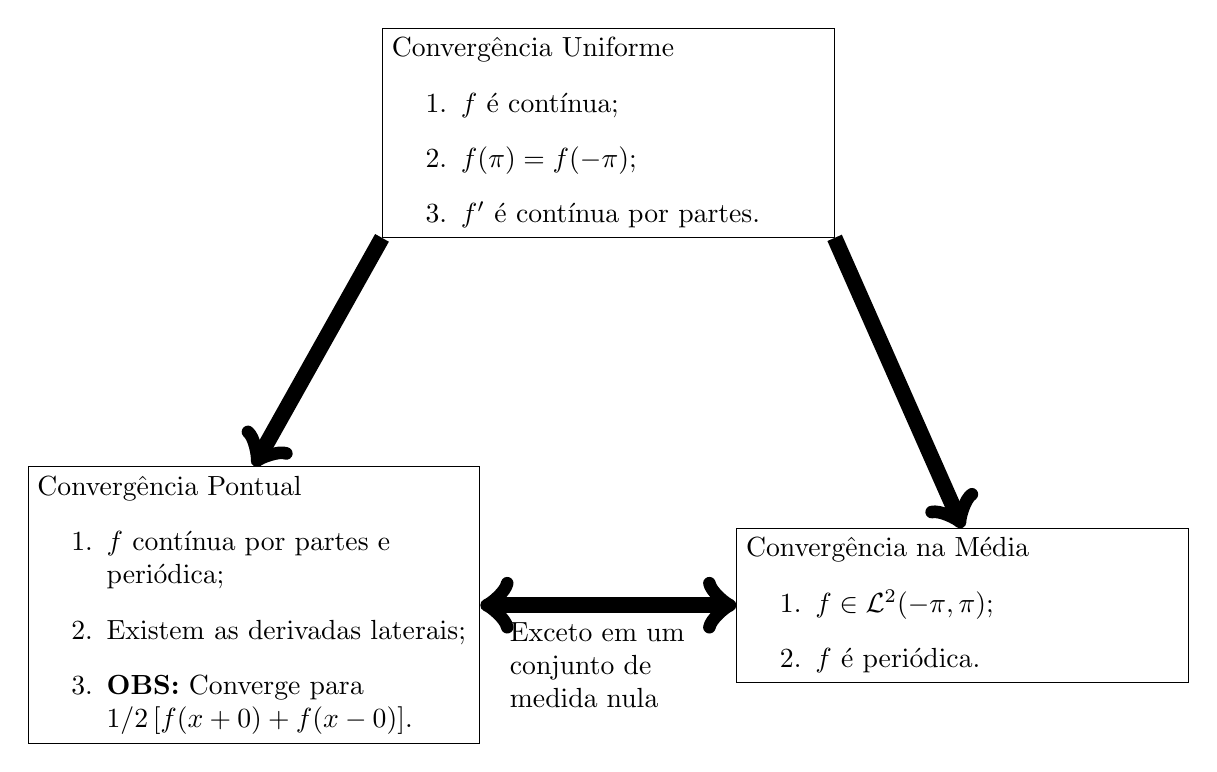
\begin{tikzpicture}
    \node[draw=black, text width=5.5cm] (U) at (0,0) {Convergência Uniforme
    \begin{enumerate}
      \item $f$ é contínua;
      \item $f(\pi) = f(-\pi)$;
      \item $f'$ é contínua por partes.
    \end{enumerate}};
    \node[draw=black, text width=5.5cm] (P) at (-4.5,-6) {Convergência Pontual
    \begin{enumerate}
      \item $f$ contínua por partes e periódica;
      \item Existem as derivadas laterais;
      \item \textbf{OBS:} Converge para $1/2 \left[ f(x + 0) + f(x - 0) \right]$.
    \end{enumerate}};
    \node[draw=black, text width=5.5cm] (M) at (4.5,-6) {Convergência na Média
    \begin{enumerate}
      \item $f \in \mathcal{L}^2(-\pi, \pi)$;
      \item $f$ é periódica.
    \end{enumerate}};
    \draw[->, line width=.2cm] (U.south west) -- (P.north);
    \draw[->, line width=.2cm] (U.south east) -- (M.north);
    \draw[<->, line width=.2cm] (P.east) -- (M.west) node[midway, below, text
    width=2.5cm] {Exceto em um conjunto de medida nula};
  \end{tikzpicture}
\end{center}

\section{Método de Fejér}
\begin{defi}
  Dadas as somas parciais $S_k(x) = \sum_{i = 0}^k \mu_i(x)$ para $k = 0, 1,
  \ldots, N - 1$, a soma de Cesàro (ou média C-1) é definida como a meia
  aritmética dessas somas parciais:
  \begin{dmath*}
    \sigma_N(x) = \frac{1}{N} \sum_{k = 0}^{N - 1} S_k(x).
  \end{dmath*}
  Dizemos que uma série é C-1 somável se existir o $\lim_{N \to \infty}
  \sigma_N(x)$.
\end{defi}
\begin{obs}
  Podemos definir a média C-2, etc, como a média aritmética das somas de
  Cesàro, ou seja,
  \begin{dmath*}
    \sigma_N^{(2)}(x) = \frac{1}{N} \sum_{k = 0}^{N - 1} \sigma_N(x),
  \end{dmath*}
  e dizer que a série é C-2 somável se existir $\lim_{N \to \infty}
  \sigma_N^{(2)}(x)$.
\end{obs}
\begin{exem}
  Considere $S_k(x) = \sum_{i = 0}^{k - 1} (-1)^i$, então
  \begin{dgroup*}
    \begin{dmath*}
      S_0 = 1,
    \end{dmath*}
    \begin{dmath*}
      S_1 = 1 - 1 = 0,
    \end{dmath*}
    \begin{dmath*}
      S_2 = 1 - 1 + 1 = 1, \vdots
    \end{dmath*}
  \end{dgroup*}
  e
  \begin{dgroup*}
    \begin{dmath*}
      S_0 = 1,
    \end{dmath*}
    \begin{dmath*}
      S_0 + S_1 = 1,
    \end{dmath*}
    \begin{dmath*}
      S_0 + S_1 + S_2 = 2, \ldots
    \end{dmath*}
  \end{dgroup*}
  Logo,
  \begin{dgroup*}
    \begin{dmath*}
      \sigma_0 = \frac{1}{1} 1 \hiderel{=} 1,
    \end{dmath*}
    \begin{dmath*}
      \sigma_1 = \frac{1}{2} 1 \hiderel{=} \frac{1}{2},
    \end{dmath*}
    \begin{dmath*}
      \sigma_2 = \frac{1}{3} 2 \hiderel{=} \frac{2}{3},
    \end{dmath*}
    \begin{dmath*}
      \sigma_3 = \frac{1}{4} 2 \hiderel{=} \frac{1}{2},
    \end{dmath*}
    \begin{dmath*}
      \sigma_4 = \frac{1}{5} 3 \hiderel{=} \frac{3}{5},
    \end{dmath*}
    \begin{dmath*}
      \sigma_5 = \frac{1}{6} 3 \hiderel{=} \frac{1}{2}, \ldots
    \end{dmath*}
    \begin{dmath*}
      \sigma_{2n} = \frac{n + 1}{2n + 1},
    \end{dmath*}
    \begin{dmath*}
      \sigma_{2n + 1} = \frac{1}{2}.
    \end{dmath*}
  \end{dgroup*}
  e como
  \begin{dgroup*}
    \begin{dmath*}
      \lim_{n \to \infty} \sigma_{2n + 1} = 1/2,
    \end{dmath*}
    \begin{dmath*}
      \lim_{n \to \infty} \sigma_{2n} = 1/2,
    \end{dmath*}
  \end{dgroup*}
  temos que a série $\sum_{i = 0}^\infty (-1)^i$ é C-1 somável e o resultado é
  $1/2$.
\end{exem}
\begin{obs}
  Usar a soma de Cesàro da série de Fourier.
  \begin{dgroup*}
    \begin{dmath*}
      \sigma_1 = \frac{a_0}{2},
    \end{dmath*}
    \begin{dmath*}
      \sigma_2 = \frac{1}{2} \left[ \frac{a_0}{2} + \left[ \frac{a_0}{2} +
      \left( a_1 \cos\left( x \right) + b_1 \sin\left( x \right) \right) \right]
      \right],
    \end{dmath*}
    \begin{dmath*}
      \sigma_3 = \frac{1}{3} \left[ \frac{a_0}{2} + \left[ \frac{a_0}{2} +
      \sum_{k = 1}^1 \left( a_k \cos\left( k x \right) + b_k \sin\left( k x
      \right) \right) \right] + \left[ \frac{a_0}{2} + \sum_{k = 1}^2 \left( a_k
      \cos\left( k x \right) + b_k \sin\left( k x \right) \right) \right]
      \right],
    \end{dmath*}
    \begin{dmath*}
      \sigma_N = \frac{1}{N} \left[ \frac{a_0}{2} + \left[ \frac{a_0}{2} +
      \sum_{k = 1}^1 \left( a_k \cos\left( k x \right) + b_k \sin\left( k x
      \right) \right) \right] \left[ \frac{a_0}{2} + \sum_{k = 1}^2 \left( a_k
      \cos\left( k x \right) + b_k \sin\left( k x \right) \right) \right]
      \vdots + \left[ \frac{a_0}{2} + \sum_{k = 1}^{N - 1} \left( a_k
      \cos\left( k x \right) + b_k \sin\left( k x \right) \right)
      \right]\right]
      = \left( \frac{N}{N} \right) \left( \frac{a_0}{2} \right) + \left(
      \frac{N - 1}{N} \right) \left( a_1 \cos\left( x \right) + b_1 \sin\left(
      x \right) \right) + \left( \frac{N - 2}{N} \left( a_2 \cos\left( 2 x
      \right) + b_2 \sin\left( 2 x \right) \right) \right) + \cdots + \left(
      \frac{N - \left( N - 1 \right)}{N} \right) \left( a_{N - 1} \cos\left(
      \left( N - 1 \right) x \right) + b_{N - 1} \sin\left( \left( N - 1
      \right) x \right) \right)
    \end{dmath*}
  \end{dgroup*}
  Portanto,
  \begin{dgroup*}
    \begin{dmath*}
      \sigma_N(x) = \frac{a_0}{2} + \sum_{k = 1}^{N - 1} \left( \alpha_k^N
      \cos\left( k x \right) + \beta_k^N \sin\left( k x \right) \right),
    \end{dmath*}
    \begin{dmath*}
      \alpha_k^N = \left( 1 - \frac{k}{N} \right) a_k,
    \end{dmath*}
    \begin{dmath*}
      \beta_k^N = \left( 1 - \frac{k}{N} \right) b_k.
    \end{dmath*}
  \end{dgroup*}

  Por outro lado, sabemos que
  \begin{dmath*}
    S_N(x) = \int_{-\pi}^\pi f(\xi) D_N(\xi - x) \vi{\xi},
  \end{dmath*}
  onde $D_N$ denota o núcleo de Dirichlet. Logo
  \begin{dmath*}
    \sigma_N(x) = \frac{1}{N} \sum_{k = 0}^{N - 1} \int_{-\pi}^\pi f(\xi)
    D_k(\xi - x) \vi{\xi}
  \end{dmath*}
  ou ainda
  \begin{dmath*}
    \sigma_N(x) = \int_{-\pi}^\pi f(\xi) F_N(\xi - x) \vi{\xi},
  \end{dmath*}
  onde
  \begin{dmath*}
    F_N(\mu) = \frac{1}{N} \sum_{k = 0}^{N - 1} D_k(\mu).
  \end{dmath*}

  Lembrando que $D_k(\mu) = \left[ \sin\left( k + 1/2 \right) \mu \right] /
  \left[ 2 \pi \sin\left( \mu/2 \right) \right]$, temos
  \begin{dmath*}
    \sin^2\left( \frac{\mu}{2} \right) F_N(\mu) = \frac{1}{N} \sin^2\left( \mu/2 \right)
    \sum_{k = 0}^{N - 1} \frac{\sin\left( k + 1/2 \right) \mu}{2 \pi \sin\left(
    \mu/2 \right)}
    = \frac{1}{2 \pi N} \sum_{k = 0}^{N - 1} \sin\left( \mu/2 \right) \sin\left(
    k + 1/2 \right) \mu
    = \frac{1}{2 \pi N} \sum_{k = 0}^{N - 1} \frac{1}{2} \left[ \cos\left( k +
    1/2 - 1/2 \right) \mu - \cos\left( k + 1/2 + 1/2 \right) \mu \right]
    = \frac{1}{4 \pi N} \sum_{k = 0}^{N - 1} \left( \cos\left( k \mu \right) -
    \cos\left( \left( k + 1 \right) \mu \right) \right)
    = \frac{1}{4 \pi N} \left( 1 - \cos\left( N \mu \right) \right)
    = \frac{1}{2 \pi N} \left( \frac{1 - \cos\left( N \mu \right)}{2} \right)
    = \frac{1}{2 \pi N} \sin^2\left( N \mu / 2 \right).
  \end{dmath*}
\end{obs}
\begin{defi}
  O núcleo de Fejér $F_N(\mu)$ é definido como
  \begin{dmath*}
    F_N(\mu) = \frac{1}{N} \sum_{k = 0}^{N - 1} D_k(\mu) = \frac{\sin^2\left( N
    \mu / 2 \right)}{2 \pi N \sin^2\left( \mu/2 \right)}.
  \end{dmath*}
\end{defi}

Antes de prosseguir, é importante notermos que:
\begin{lem}
  Temos que
  \begin{dgroup*}
    \begin{dmath*}
      \int_{-\pi}^\pi D_k(\mu) \vi{\mu} = 1,
    \end{dmath*}
    \begin{dmath*}
      \int_{-\pi}^\pi F_k\left( \mu \right) \vi{\mu} = 1.
    \end{dmath*}
  \end{dgroup*}
\end{lem}
\begin{proof}
  Sabendo que
  \begin{dmath*}
    D_k(\mu) = \frac{\sin\left( k + 1/2 \right) \mu}{2 \pi \sin\left( \mu/2
    \right)}
    = \left( 1 + 2 \sum_{j = 1}^{k - 1} \cos\left( j \mu \right) \right)
    \frac{1}{2 \pi}
  \end{dmath*}
  temos que
  \begin{dmath*}
    \int_{-\pi}^\pi D_k\left( \mu \right) \vi{\mu} = \frac{1}{2 \pi} \left[ \pi
    - \left( -\pi \right) + 2 \sum_{j = 1}^{k - 1} \left. \frac{\sin\left( j \mu
    \right)}{j} \right|_{-\pi}^\pi \right] = 1
  \end{dmath*}
  e
  \begin{dmath*}
    \int_{-\pi}^\pi F_k(\mu) \vi{\mu} = \frac{1}{k} \sum_{j = 0}^{k - 1}
    \int_{-\pi}^\pi D_j(\mu) \vi{\mu} = \frac{1}{k} k = 1. \qedhere
  \end{dmath*}
\end{proof}
\begin{teo}[Fejér] \label{teo:fejer}
  Seja $f(x)$ uma função contínua e periódica (de período $2\pi$) e seja
  $\sigma_N(x)$ a soma de Cesàro da série de Fourier de $f(x)$, ou seja,
  \begin{dmath*}
    \sigma_N(x) = \frac{a_0}{2} + \sum_{k = 1}^{N - 1} \left( \alpha_k^N
    \cos\left( k x \right) + \beta_k^N \sin\left( k x \right) \right),
  \end{dmath*}
  onde $\sigma_k^N = \left( 1 - k/N \right) a_k$ e $\beta_k^N = \left( 1 - k/N
  \right) b_k$. Então a sequência de funções $\sigma_n(x)$ converge para $f(x)$.
\end{teo}
\begin{proof}
  (mais fácil que Fourier pois $F_N(\mu) \geq 0$)
  \begin{dgroup*}
    \begin{dmath*}
      \sigma_N(x) = \int_{-\pi}^\pi f(\xi) F_N(\xi - x) \vi{\xi}
      = \int_{a - \pi}^{a + \pi} f(\xi) F_{N}(\xi - x) \vi{\xi}
      = \int_{x - \pi}^{x + \pi} f(\xi) F_N(\xi - x) \vi{\xi}
      = \int_{-\pi}^\pi f(x + \mu) F_N(\mu) \vi{\mu}
    \end{dmath*}
    \begin{dmath*}
      \sigma_N(x) - f(x) = \int_{-\pi}^\pi f(x + \mu) F_N(\mu) \vi{\mu} - f(x)
      \int_{-\pi}^\pi F_N(\mu) \vi{\mu}
      = \int_{-\pi}^\pi \left[ f(x + \mu) - f(x) \right] F_N(\mu) \vi{\mu}
      = \frac{1}{\pi N} \int_{-\pi}^\pi \left[ f(x + \mu) - f(x) \right]
      \frac{\sin^2\left( N \mu/2 \right)}{2 \sin^2\left( \mu/2 \right)} \vi{\mu}
    \end{dmath*}
  \end{dgroup*}
  Logo, como $f$ é contínua então $\forall \epsilon > 0, \exists \delta > 0$ tal
  que $| f(x + \mu) - f(x)| < \epsilon$ para $| x + \mu - x| = | \mu | <
  \delta$.
  \begin{dmath*}
    \left\| \sigma_N(x) - f(x) \right\| = \left| \int_{-\pi}^\pi \left( \ldots \right) \right|
    = \left| \int_{-\pi}^{-\delta} \left( \ldots \right) + \int_{-\sigma}^\sigma
    \left( \ldots \right) + \int_\sigma^\pi \left( \ldots \right) \right|
    \leq \underbrace{\left| \int_{-\pi}^{-\delta} \left( \ldots \right)
    \right|}_{|I_1|} + \underbrace{\left| \int_{-\sigma}^\sigma \left( \ldots
    \right) \right|}_{|I_2|} + \underbrace{\left| \int_\sigma^\pi \left( \ldots
    \right) \right|}_{|I_3|}
  \end{dmath*}
  Mas
  \begin{dgroup*}
    \begin{dmath*}
      \left\| I_2 \right\| \leq \int_{-\delta}^\delta \underbrace{| f(x + \mu) - f(x) |}_{< \epsilon} F_N(\mu) \vi{\mu}
      < \epsilon \int_{-\delta}^\delta \underbrace{F_N(\mu)}_{\geq 0} \vi{\mu}
      < \epsilon \underbrace{\int_{-\delta}^\delta F_N(\mu) \vi{\mu}}_{=1}
      < \epsilon,
    \end{dmath*}
    \begin{dmath*}
      \left\| I_1 \right\| \leq  \frac{1}{\pi N} \int_{-\pi}^{-\delta} | f(x + \mu) - f(x) |
      \frac{\sin^2\left( N \mu/2 \right)}{2 \sin^2\left( \mu/2 \right)} \vi{\mu}
      \leq \frac{2 M}{\pi N} \int_{-\pi}^{-\delta} \frac{\sin^2\left( N \mu/2
      \right)}{2 \sin^2\left( \mu/2 \right)} \vi{\mu}
      \intertext{onde $M = \max |f(x)|$}
      \leq \frac{2 M}{\pi N} \int_{-\pi}^{-\delta} \frac{1}{2 \sin^2\left( \mu/2
      \right)} \vi{\mu}
      \leq \frac{2 M}{\pi N} \int_{-\pi}^{-\delta} \frac{1}{2 \sin^2\left(
      \delta/2 \right)} \vi{\mu}
      = \frac{M}{\pi N \sin^2\left( \delta/2 \right)}
      \underbrace{\int_{-\pi}^{-\delta} \vi{\mu}}_{\pi - \delta < \pi}
      \leq \frac{M \pi}{\pi N \sin^2\left( \delta/2 \right)}
      \leq \frac{M}{N \sin^2\left( \delta/2 \right)},
      \intertext{e analogamente}
    \end{dmath*}
    \begin{dmath*}
      \left\| I_3 \right\| \leq \frac{M}{N \sin^2\left( \delta/2 \right)}.
    \end{dmath*}
  \end{dgroup*}
  Portanto,
  \begin{dgroup*}
    \begin{dmath*}
      |\sigma_N(x) - f(x)| \leq \epsilon + \frac{2 M}{N \sin^2\left( \delta/2 \right)},
    \end{dmath*}
    \begin{dmath*}
      \lim_{N \to \infty} | \sigma_N(x) - f(x) | \leq \epsilon
    \end{dmath*}
  \end{dgroup*}
  de onde concluímos que
  \begin{dmath*}
    \lim_{N \to \infty} \sigma_N(x) = f(x) \qedhere
  \end{dmath*}
\end{proof}

\section{Diferenciação e Integração}
\begin{teo}
  Seja $f(x)$ uma função contínua em $[-\pi,\pi]$ tal que $f(-\pi) = f(\pi)$ e
  seja $f'(x)$ contínua por partes e com derivadas laterais nesse intervalo.
  Então a série de Fourier de $f(x)$ é diferenciável e
  \begin{dmath*}
    f'(x) = \sum_{n = 1}^\infty n \left( -a_n \sin\left( n x \right) + b_n
    \cos\left( n x \right) \right)
  \end{dmath*}
\end{teo}
\begin{proof}
  Como $f'(x)$ satisfaz as condições do Teorema de Fourier
  (página~\pageref{teo:fourier}), ela possui a série de Fourier
  \begin{dmath*}
    f'(x) = \frac{\alpha_0}{2} + \sum_{n = 1}^\infty \left( \alpha_n \cos\left(
    n x \right) + \beta_n \sin\left( n x \right) \right).
  \end{dmath*}
  Mas
  \begin{dgroup*}
    \begin{dmath*}
      \alpha_0 = \frac{1}{\pi} \int_{-\pi}^\pi f'(x) \vi{x}
      = \frac{1}{\pi} \left[ f(\pi) - f(-\pi) \right]
      = 0,
    \end{dmath*}
    \begin{dmath*}
      \alpha_n = \frac{1}{\pi} \left[ \underbrace{\left. f(x) \cos\left( n x
      \right) \right|_{-\pi}^\pi}_{=0} + n \int_{-\pi}^\pi f(x) \sin\left( n x
      \right) \vi{x} \right]
      = n b_n
    \end{dmath*}
    \begin{dmath*}
      \beta_n = \frac{1}{\pi} \left[ \underbrace{\left. f(x) \sin\left( n x
      \right) \right|_{-\pi}^\pi}_{=0} - n \int_{-\pi}^\pi f(x) \cos\left( n x
      \right) \vi{x} \right]
      = -n a_n
    \end{dmath*}
  \end{dgroup*}
  de modo que
  \begin{dmath*}
    f'(x) = \sum_{n = 1}^\infty \left( n b_n \cos\left( n x \right) - n a_n
    \sin\left( n x \right) \right). \qedhere
  \end{dmath*}
\end{proof}
\begin{obs}
  Note que o teorema fornece apenas uma condição suficiente. Além disso, podemos
  ter série de Fourier para $f(x)$ e não para $f'(x)$ (nesse caso o termo $n$ no
  numerador diminui a taxa de convergência da série).
\end{obs}
\begin{exem}
  A função $f(x) = x$ possui a série de Fourier
  \begin{dmath*}
    x = 2 \sum_{n = 1}^\infty (-1)^{n + 1} \frac{\sin\left( n x \right)}{n}.
  \end{dmath*}
  Porém $f(-\pi) = -\pi \neq \pi f(\pi)$, de modo que as condições do teorema
  não são satisfeitas e nada podemos afirmar acerca da série de Fourier de
  $f'(x)$ usando esse teorema. Note que nesse caso que a derivada da série de
  Fourier não converge!
  \begin{dmath*}
    1 \neq 2 \sum_{n = 1}^\infty (-1)^{n + 1} \cos\left( n x \right).
  \end{dmath*}
\end{exem}
\begin{obs}
  Dentro das condições do teorema anterior, uma vez que $\lim_{n \to \infty}
  \alpha_n = 0$ e $\lim_{n \to \infty} \beta_n = 0$ (critério do termo geral),
  temos
  \begin{dgroup*}
    \begin{dmath*}
      \lim_{n \to \infty} n a_n = 0,
    \end{dmath*}
    \begin{dmath*}
      \lim_{n \to \infty} n b_n = 0.
    \end{dmath*}
  \end{dgroup*}
  Note que a série do exemplo anterior não satisfaz essas condições.
\end{obs}
\begin{teo}
  Seja $f(x)$ uma função contínua por partes em $(-\pi,\pi)$. Então,
  independentemente da série de Fourier de $f(x)$ convergir ou não, vale a
  seguinte igualdade:
  \begin{dmath*}
    \int_{-\pi}^x f(\xi) \vi{\xi} = \frac{1}{2} a_0 \left( x + \pi \right) +
    \sum_{n = 1}^\infty \frac{1}{n} \left[ a_n \sin\left( n x \right) - b_n
    \left( \cos\left( n x \right) - \cos\left( n \pi \right) \right) \right],
  \end{dmath*}
  quando $x \in [-\pi,\pi]$.
\end{teo}
\begin{proof}
  Seja
  \begin{dmath*}
    F(x) = \int_{-\pi}^x f(\xi) \vi{\xi} - \frac{a_0}{2} x.
  \end{dmath*}
  Se $f(x)$ é contínua por partes então $F(x)$ é contínua. Além disso $F'(x) =
  f(x) - a_0/2$, de modo que $F'(x)$ é contínua por partes. Podemos ainda notar
  que $F(-\pi) = -a_0 / 2 (-\pi) = \pi a_0 / 2$ e
  \begin{dmath*}
    F(\pi) = \int_{-\pi}^\pi f(\xi) \vi{\xi} - \frac{a_0}{2} \pi
    = a_0 \pi - \frac{a_0}{2} \pi
    = \frac{a_0 \pi}{2}
  \end{dmath*}
  ou seja, $F(\pi) = F(-\pi)$. Temos com isso que $F(x)$ satisfaz as condições
  do teorema de Fourier e possui portanto a série de Fourier
  \begin{dgroup*}
    \begin{dmath*}
      F(x) = \frac{A_0}{2} + \sum_{n = 1}^\infty \left( A_n \cos\left( n x
      \right) + B_n \sin\left( n x \right) \right),
    \end{dmath*}
    \begin{dmath*}
      A_n = \frac{1}{\pi} \int_{-\pi}^\pi F(x) \cos\left( n x \right) \vi{x},
    \end{dmath*}
    \begin{dmath*}
      B_n = \frac{1}{\pi} \int_{-\pi}^\pi F(x) \sin\left( n x \right) \vi{x}.
    \end{dmath*}
  \end{dgroup*}
  Para $n \neq 0$,
  \begin{dgroup*}
    \begin{dmath*}
      A_n = \frac{1}{n} \int_{-\pi}^\pi \left[ \int_{-\pi}^x f(\xi) \id(\xi) -
      \frac{a_0}{2} x \right] \cos\left( n x \right) \vi{x}
      = \frac{1}{\pi} \underbrace{\left. F(x) \frac{\sin\left( n x \right)}{n}
      \right|_{-\pi}^\pi}_{=0} - \frac{1}{\pi} \int_{-\pi}^\pi \frac{\sin\left(
      n x \right)}{n} \left[ f(x) - \frac{a_0}{2} \right] \vi{x}
      = - \frac{1}{n \pi} \int_{-\pi}^\pi f(x) \sin\left( n x \right) \vi{x} +
      \frac{a_0}{2 n \pi} \underbrace{\int_{-\pi}^\pi \sin\left( n x \right)
      \vi{x}}_{=0}
      = -\frac{1}{n} b_n,
    \end{dmath*}
    \begin{dmath*}
      B_n = \frac{1}{n} \int_{-\pi}^\pi \left[ \int_{-\pi}^x f(\xi) \vi{\xi} -
      \frac{a_0 x}{2} \right] \sin\left( n x \right) \vi{x}
      = \underbrace{-\frac{1}{\pi} \left. F(x) \frac{\cos\left( n x \right)}{n}
      \right|_{-\pi}^\pi}_{=0} + \frac{1}{n \pi} \int_{-\pi}^\pi \cos\left( n x
      \right) \left[ f(x) - \frac{a_0}{2} \right] \vi{x}
      = \frac{1}{n \pi} \int_{-\pi}^\pi \cos\left( n x \right) f(x) \vi{x} -
      \frac{a_0}{2 n \pi} \underbrace{\int_{-\pi}^\pi \cos\left( n x \right)
      \vi{x}}_{=0}
      = \frac{1}{n} a_n
    \end{dmath*}
  \end{dgroup*}
  e portanto
  \begin{dmath*}
    F(x) = \frac{A_0}{2} + \sum_{n = 1}^\infty \left( \frac{-b_n}{n} \cos\left(
    n x \right) + \frac{a_n}{n} \sin\left( n x \right) \right).
  \end{dmath*}
  Tomando $x = \pi$,
  \begin{dmath*}
    F(\pi) = \frac{a_0 \pi}{2} = \frac{A_0}{2} \sum_{n = 1}^\infty \left(
    \frac{-b_n}{n} \cos\left( n \pi \right) + \frac{a_n}{n}
    \underbrace{\sin\left( n \pi \right)}_{=0} \right)
  \end{dmath*}
  e portanto
  \begin{dmath*}
    \frac{A_0}{2} = \frac{a_0 \pi}{2} + \sum_{n = 1}^\infty \frac{b_n}{n}
    \cos\left( n \pi \right)
  \end{dmath*}
  de modo que
  \begin{dmath*}
    \int_{-\pi}^x f(\xi) \vi{\xi} - \frac{a_0 x}{2} = \frac{a_0 \pi}{2} +
    \sum_{n = 1}^\infty \frac{1}{n} \left[ a_n \sin\left( n x \right) - b_n
    \left( \cos\left( n x \right) - \cos\left( n \pi \right) \right) \right].
    \qedhere
  \end{dmath*}
\end{proof}
\begin{obs}
  Note que no caso da integração o termo $n$ no denominador aumenta a taxa de
  convergência.
\end{obs}
\begin{exem}
  A série de $f(x) = x$ é
  \begin{dmath*}
    x = 2 \sum_{n = 1}^\infty (-1)^{n + 1} \frac{\sin\left( n x \right)}{n}.
  \end{dmath*}
  Tomando $\int_0^x f(\xi) \vi{\xi}$ temos
  \begin{dmath*}
    x^2 = 4 \sum_{n = 1}^\infty \frac{(-1)^n}{n^2} \cos\left( n x \right) - 4
    \sum_{n = 1}^\infty \frac{(-1)^n}{n^2}
  \end{dmath*}
  que é justamente a série obtida na página~\pageref{exem:fourier:x^2} uma vez
  que $\sum_{n = 1}^\infty (-1)^n / (n^2) = -\pi^2 / 12$.
\end{exem}

\section{Fenômeno de Gibbs}
Para ilustrar o fenômeno de Gibbs, vamos considerar uma onda quadrada periódica
representada por
\begin{dmath*}
  f(x) = \begin{cases}
    h/2, & 0 < x < \pi, \\
    -h/2, & -\pi < x < 0.
  \end{cases}
\end{dmath*}
e ilustrada na Figura
\begin{figure}[!htb]
  \centering
  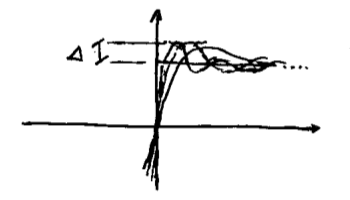
\includegraphics[width=.5\textwidth]{figuras/05-0}
  \begin{flushright}
    Imagem em domínio público de Johannes Rössel e disponível em
    \url{http://en.wikipedia.org/wiki/File:Gibbs_phenomenon_10.svg}.
  \end{flushright}
  \caption{Ilustração do Fenômeno de Gibbs para onda quadrada.}
  \label{fig:fenom_gibbs}
\end{figure}
% TODO Terminar de digitar a seção sobre o Fenômeno de Gibbs do arquivo M2S12-5.

\section{Teorema da Aproximação de Weierstrass}
\begin{teo}
  Seja $f(x)$ contínua em $a \leq x \leq b$. Então para todo $\epsilon > 0$
  existe um polinômio $P(x)$ tal que $|P(x) - f(x)| \leq \epsilon, \forall x \in
  [a,b]$.
\end{teo}
\begin{proof}
  Dado $f(x)$, $x \in [a,b]$, podemos definir $g(t)$ para $t \in [-\pi/2,
  \pi/2]$ através de
  \begin{dmath*}
    g(t) = f\left[ \left( \frac{b - a}{\pi} t + \left( \frac{b - a}{2} \right)
    \right) \right].
  \end{dmath*}
  Podemos ainda definir uma extensão de $g(t)$ para $x \in [-\pi, \pi]$, que
  denotaremos por $G(t)$, e de modo que $G(-\pi) = G(\pi)$. Podemos além disso
  considerar para os demais pontos a extensão periódica de $G(t)$. Nessas
  condições o Teorema de Fejér (página~\pageref{teo:fejer}) nos garante que a
  sequência $\sigma_N(t)$,
  \begin{dmath*}
    \sigma_N(t) = \frac{a_0}{2} + \sum_{k = 1}^{N - 1} \left( \alpha_k^N
    \cos\left( k t \right) + \beta_k^N \sin\left( k t \right) \right),
  \end{dmath*}
  converge para $G(t)$, ou seja, $\forall \epsilon > 0$, existe $N_0 > 0$ tal
  que
  \begin{dmath*}
    | \sigma_N(t) - G(t) | < \epsilon/2
  \end{dmath*}
  para $N > N_0$. Por outro lado, pelo Teorema de Taylor, existem polinômios
  $R_n^k(t)$ e $S_n^k(t)$ de grau $n$ tais que
  \begin{dgroup*}
    \begin{dmath*}
      | \cos\left( k t \right) - R_n^k(t) | < \epsilon',
    \end{dmath*}
    \begin{dmath*}
      | \sin\left( k t \right) - S_n^k(t) | < \epsilon'',
    \end{dmath*}
  \end{dgroup*}
  para $n > N_1$. Portanto, existe um polinômio $Q_N(t)$, que é uma combinação
  dos polinômios $R_n^k(t)$ e $S_n^k(t)$, tal que
  \begin{dmath*}
    | \sigma_N(t) - Q_N(t) | < \epsilon/2.
  \end{dmath*}
  Com isso,
  \begin{dmath*}
    | G(t) - Q_N(t) | = | G(t) - \sigma_N(t) + \sigma_N(t) - Q_N(t) |
    \leq \underbrace{| G(t) - \sigma_N(t) |}_{< \epsilon/2} + \underbrace{|
    \sigma_N(t) - Q_N(t) |}_{< \epsilon/2}
  \end{dmath*}
  e portanto $| G(t) - Q_N(t) | < \epsilon$ para $t \in [-\pi, \pi]$ e $| g(t) -
  Q_N(t) | < \epsilon$ para $t \in [-\pi/2, \pi/2]$ ou, definindo $P_N(x) =
  Q_N\left[ \left( \pi / \left( b - a \right) \right) x - \left( \pi / 2 \right)
  \left( \left( b + a \right) / \left( b - a \right) \right) \right]$,
  \begin{dmath*}
    | f(x) - P_N(x) | < \epsilon
  \end{dmath*}
  para $x \in [a, b]$.
\end{proof}
